\graphicspath{ {./Chapter 2/figures/} {./Chapter 2/figures/Snake/} {./Chapter 2/figures/Water/} {./Chapter 2/results/} }

\chapter{Semantic terrain representation}
\label{chap:semantic-representation}
\teaser{
\includegraphics[width=0.9\linewidth]{figureTeaser.png}
% % \centering
% \caption{Our method can produce different scenes including coral reef islands and canyons at multiple scales using \glosses{EnvObj} to represent terrain features.}
\label{fig:env-obj-teaser}
\caption{Three underwater scenes using our \glosses{EnvObj} representation. From left to right: an island cut in half by a canyon, the inside of a canyon with rocks and corals, an island with corals, algae and a trench.}
}

\abstract
\label{chap:env-obj-abstract}
This chapter introduces a novel method for procedural terrain generation, which leverages a sparse representation of environmental features to produce landscapes that are lightweight, plausible and adaptable to user desires. The method differs from traditional terrain generation approaches by emphasising multi-scale user interaction and incorporating expert knowledge to model the evolution of terrain features over time. By representing terrain features as discrete entities, or "\glosses{EnvObj}", the method enables dynamic interaction between these entities and their surrounding environment, represented through continuous scalar and vector fields. The generation process is iterative and allows for user-guided modifications at any iteration, including the introduction of environmental events that can influence the terrain's evolution. The proposed approach is particularly flexible, capable of generating underwater landscapes with a focus on large-scale plausibility and detailed, localised feature representation.
\pagebreak

\minitoc

% topography
% Representing an environment as a topographic map
% A method that uses new objects, EnvObjs, to represent the landmarks of a terrain
% Our method represents the different landmarks of a terrain using a geometric (as "without 3D repr") representation. To avoid cycles in the interactions between objects, we use the environment as a proxy. EnvObjs are independant, like cellular automata. Each object affects locally the environment by modifying EnvVals. This modifications are applied by the EnvObjs spreading EnvMat around them. They also absorb EnvMat from the other EnvObjs. We can consider that the diffusion is bounded thanks to a decay rate, meaning the system becomes stable after some time. Because it is stable, it is plausible. We break the stability by adding new EnvObjs following \glosses{GenRule}. New EnvObjs are placed in the environment where they may be the most probable, following a fitness function using the EnvVals. Then the shape of the skeleton is defined following a skeleton \gloss{FitnessFunc}. We wait for the environment to stabilise. It can take some time, and some EnvObjs might die (if fitness function falls below 0), but it will converge. The user can guide this process by defining EnvObjs that can spawn. Also, because it is a simple skeleton, he can modify shapes. The diffusion process is deterministic so no abrupt changes in the landscape. Also, the stability of the system can be broken by influencing EnvVals. So the user can affect them through \Glosses{GeoEvent}. \Glosses{GeoEvent} affect one or more EnvVal over time, but we reduce the number of evaluations to the beginning and end of the \glosses{GeoEvent}. Each EnvObj has a probability of chance to spawn each day, which can be computed as an amount per month, year, etc. (Probability Distribution Function of $p(X) = p^t$).

\section{Introduction}

Procedural ecosystem generation in computer graphics remains largely bifurcated: classical terrain algorithms produce heightfields or meshes without semantic structure, and plant-placement systems adopt fixed-radius or zone-of-influence rules for foliage alone. Meanwhile, full ecosystem simulators, though rich in biotic and abiotic processes, are too costly for real-time or interactive content creation. Consequently, no prior work combines sparse, semantic primitives for both living and non-living features, multi-material field coupling driven to steady state, and multi-scale, user-interactive authoring into a single, lightweight ecosystem generator.

To fill this gap, we introduce a pipeline that constructs both biotic (corals, algae, trees) and abiotic (islands, rivers, canyons) elements by instantiating \glosses{EnvObj} (points, curves, regions) which read from and write to continuous environmental fields (elevation, water flow, resource stocks) in an iterative, steady-state diffusion loop. At each step, \glosses{EnvObj} candidates spawn or die via expert-tuned generation and fitness rules, and users can inject global geomorphological events or manually refine any primitive, all while maintaining interactive performance for thousands of objects.


\begin{figure}
    \autofitgraphics[]{CliffErosionBidefordAndScalby.jpg, geologyMadagascar.jpeg}
     \autofitgraphics[]{QasrLibya.jpg, PerthCanyon.jpg}
    \caption{Examples of cartographies used in different fields of natural science. From left to right, and top to bottom: Evolution of coastlines at Bideford, UK and Scalby, UK over the last 6000 years and 2000 years respectively (BP = Before Present) \cite{Shadrick2022}; sedimentary distribution over Madagascar island \cite{Pratt2017}; geological features distribution of karstic landscape at Qasr Libya, Libya \cite{ElAmawy2009}; localisation of key parameters of Perth Submarine Canyon, Australia \cite{Huang2014}}
    \label{fig:env-obj-symbolics-on-maps}
\end{figure}

We draw qualitative inspiration from cartographic symbology, where topographic and bathymetric charts employ 0D points (volcanoes, observatories), 1D lines (canyon heads, reef crests), and 2D regions (soil or sediment covers) to strip away geometric complexity and preserve the spatial relationships that underpin expert reasoning (see \cref{fig:env-obj-symbolics-on-maps}). Similarly to these map primitives, our \gloss{EnvObj} abstractions enable a “sketch-first, refine-later” workflow: designers begin with a coarse semantic layout, then progressively zoom in, from mountain ridges down to individual boulders or coral colonies, without ever losing global coherence.

In the following state of the art, we first review classical radius-based heuristics used for ecosystem generation in Computer graphics (FRN, ZOI), and ecological-field theories (EFT) and reaction-diffusion that inform our local interaction and diffusion mechanisms. We then present our \glosses{EnvObj}-\glosses{EnvVal} pipeline in detail and demonstrate its use for underwater coral-reef environments. %both terrestrial mountain scenes and underwater coral-reef environments.

Unlike full-fledged ecosystem simulations, which model temporal dynamics (population growth, predator-prey interactions, nutrient cycling, and fluid flows, ...) over successive time steps to study emergent behavior, our work centers on ecosystem generation, where the goal is to produce a plausible, editable snapshot of a landscape by iteratively placing and culling semantic primitives (\glosses{EnvObj}) that read from and write to steady-state environmental fields; this generation process trades off dynamic fidelity for interactive performance and multi-scale user control, delivering plausible biotic and abiotic scene layouts without the overhead of continuous process simulation.

Building on these observations, this chapter contributes:
\begin{Itemize}
\Item{} \hide{\Gloss{EnvObj} formalism:} We introduce a sparse, domain-agnostic symbol set (points, curves, regions) that both read continuous environmental fields and write local modifications back to them, creating a closed feedback loop.

\Item{} \hide{Analytic field coupling:} A decay-stabilised reaction-diffusion solver for scalar "materials" and analytical deformation of the vector-flow field yield interactive, steady-state updates without heavy fluid or erosion simulation.

\Item{} \hide{Multi-scale authoring:} A focus-and-refine pipeline lets users jump from kilometre-scale planning to sub-metre edits while preserving global coherence. %We demonstrate this on both coral-reef islands and terrestrial mountain scenes.

\end{Itemize}








% \section{Introduction}

% % \begin{figure}%[ht]
% % 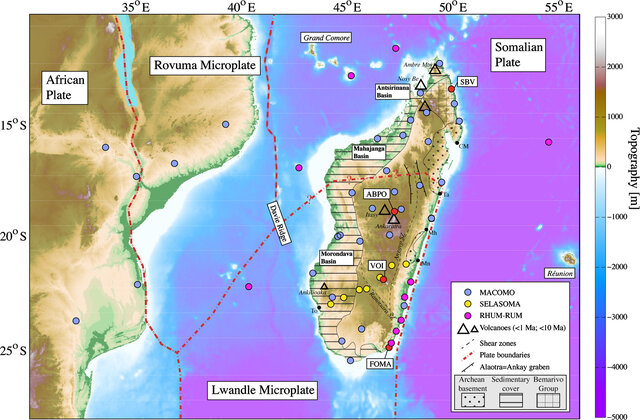
\includegraphics[width=0.5 \linewidth]{./geologyMadagascar.jpeg}
% % 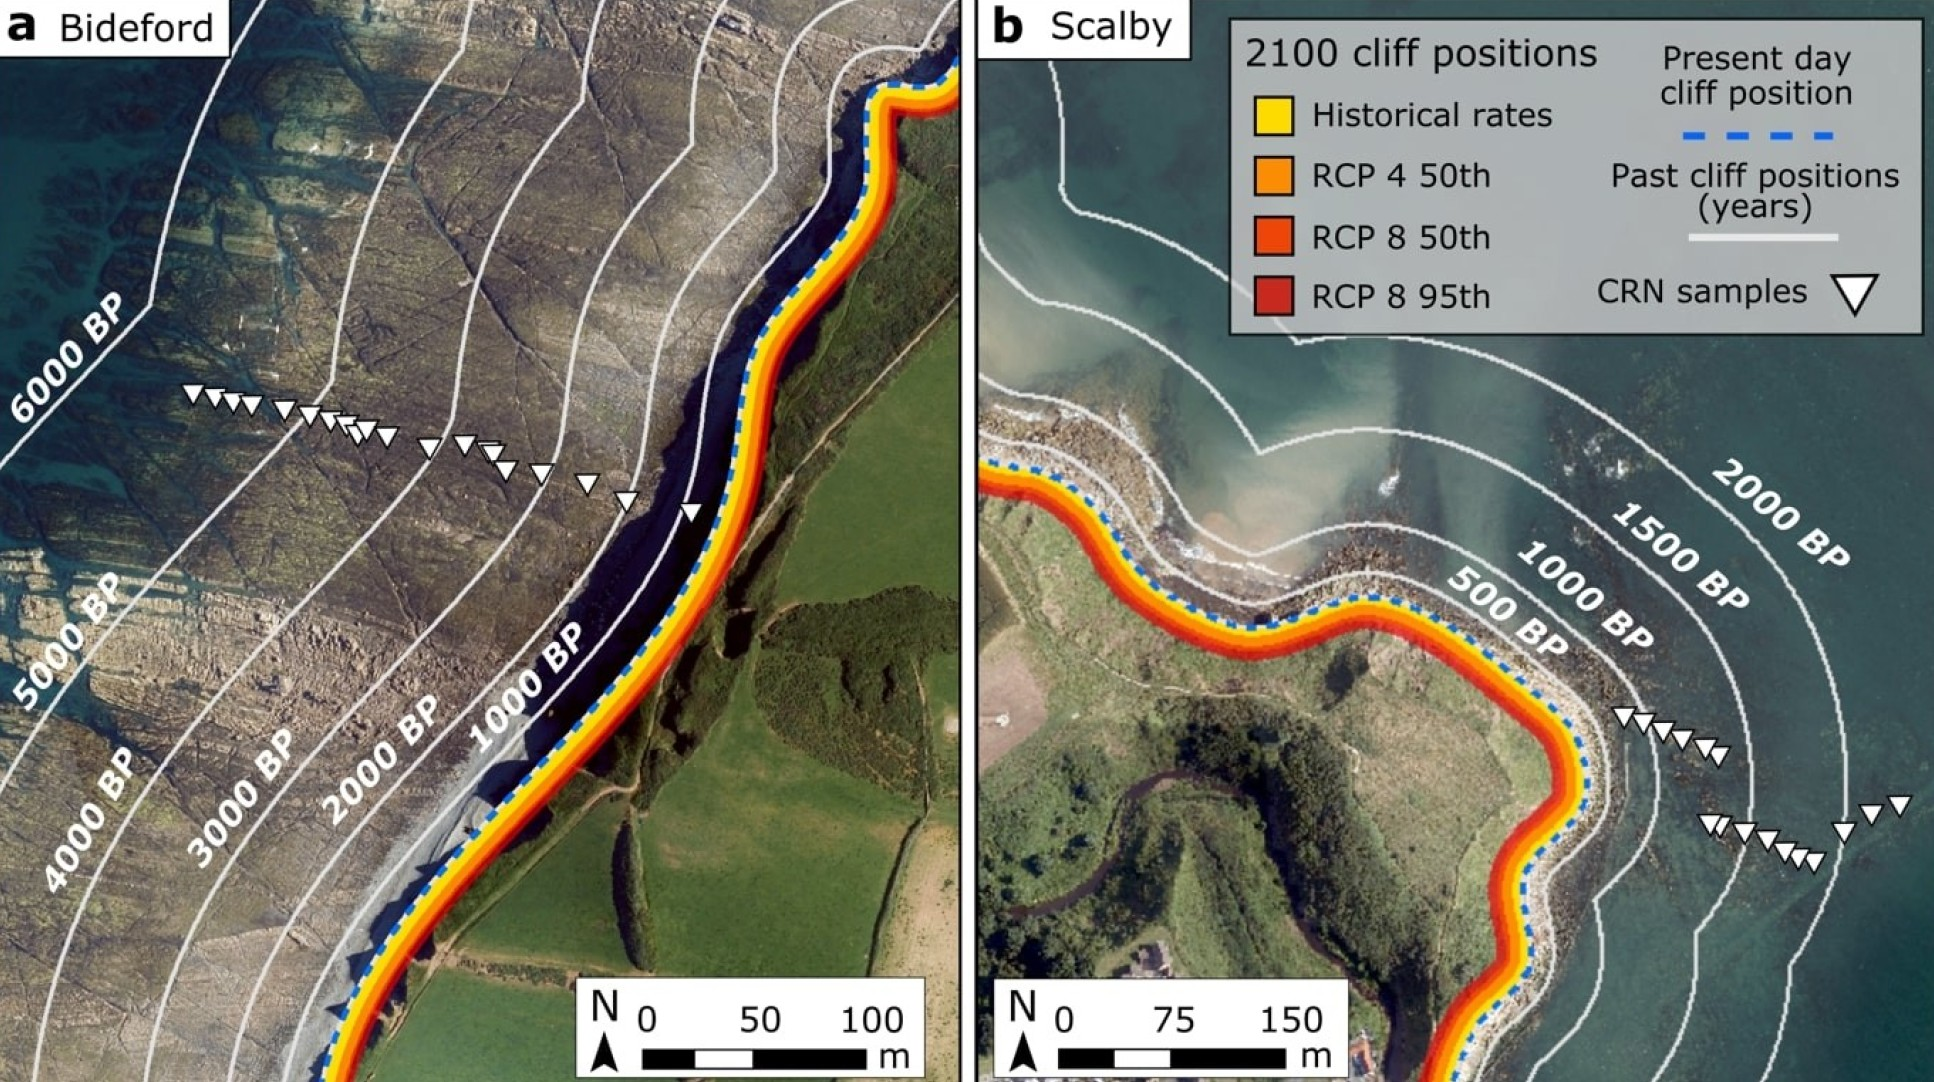
\includegraphics[width=0.5 \linewidth]{./CliffErosionBidefordAndScalby.jpg}
% % 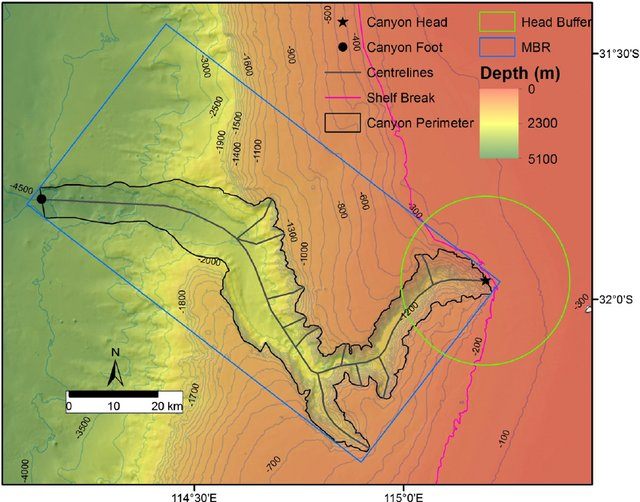
\includegraphics[width=0.5 \linewidth]{./PerthCanyon.jpg}
% % 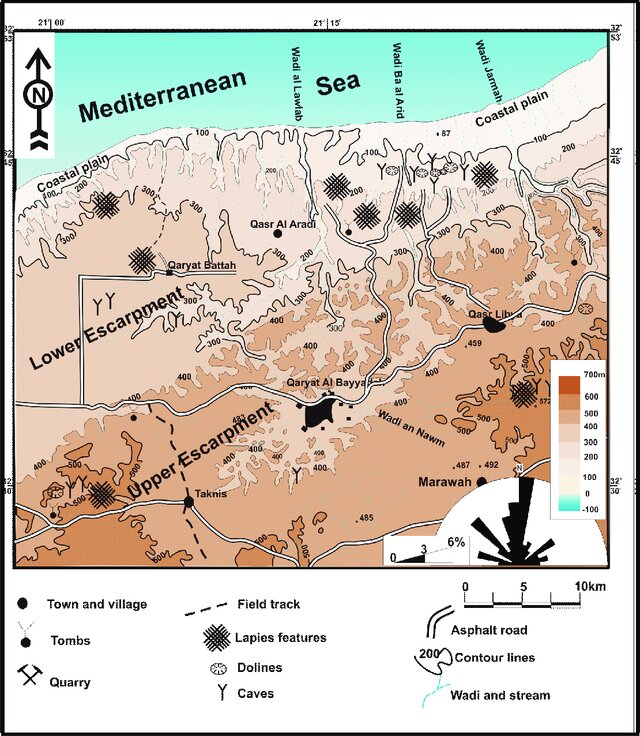
\includegraphics[width=0.5 \linewidth]{./QasrLibya.jpg}
% % \caption{Four examples of topographic maps used in earth science. From left to right and top to bottom: Sedimentary distribution off Madagascar island \cite{Pratt2017}, evolution of coastlines at Bideford, UK and Scalby, UK over the last 6000 years and 2000 years respectively (BP = Before Present) \cite{Shadrick2022}, localisation of key parameters of Perth Submarine Canyon, Australia \cite{Huang2014}, and geological features distribution of karstic landscape at Qasr Libya, Libya \cite{ElAmawy2009}}
% % \label{fig:env-obj-presentation}
% % \end{figure}

% % Slight introduction
% Virtual terrain generators often deliver raw geometry or grids, but field experts need the symbolic cues they draw on topographic or bathymetric maps (canyon heads, reef crests, dune ridges). Topographic maps are indispensable tools for biologists, geologists, or oceanologists (who refer to their sub-sea equivalents as "bathymetric charts"). These maps are displayed in 2D but provide 3D information about elevation (or depth). They can also use symbology to represent multi-scale elements that must remain legible. In cartography, map symbols are defined as geometric primitives such as points, polylines, polygons, and (more rarely) polyhedrons. Map symbols are essential compression devices: they strip away geometric detail while preserving the relationships that matter.

% This abstraction helps us grasp the relationship between different features, and can therefore enable the deduction of physical rules in the evolution of a terrain through the process of observation. In fields where full mechanistic modelling is out of reach (earth science, biology, urbanism, ...), the deduction of rules through observation plays an important role in the understanding of phenomena and explication of situations. Consequently, symbolic maps act as a cognitive bridge: they let experts infer governing processes and develop testable hypotheses even when full mechanistic simulation or controlled experiments are impossible.

% In this way, geologists can study the distribution of peaks in a mountain range or the location of soil types in an area (\cref{fig:env-obj-topo-madagascar}), which in turn helps them infer the probable locations of karst networks (\cref{fig:env-obj-topo-karst}), for example. Using the same abstraction tools, a biologist may study the effect of natural or artificial reefs on coastal erosion (\cref{fig:env-obj-topo-coasts}), or understand more clearly the interactions inside an ecosystem. Oceanologists may also deduce, in a similar manner, the formation of canyons and fans from old river systems (\cref{fig:env-obj-topo-canyon}). In short, the same minimalist notation empowers diverse fields to reason about terrain. This cross-disciplinary utility is the key inspiration for the \glosses{EnvObj} representation introduced in this chapter.

% %--- AltTextImage R (coastlines) ------------------------------------
% \AltTextImageR{%
% The use of parametric lines representing coasts of islands or continents is common because it is intuitive to understand the concept of interaction using curves. It also shows an easy way to present the evolution of this interaction with respect to time, as the continuous change of shape can be interpreted by our mind as a moving shape, providing a sense of velocity of change (\cref{fig:env-obj-topo-coasts}). While real coastlines are fractal, a representation using a continuous line is sufficient to be able to imagine the real scene. A more detailed representation would however be harder to read, without any significant improvement in interpretability, and would age quickly as the coast evolves.

% Any element, such as a coastline, then has an organic evolution over time, just like biological elements that can grow, shrink, and morph continuously. We see that one of the main differences between the evolution of organic elements, such as the borders of a forest, and non-organic elements, such as the borders of an island, lies in the time scale.
% }{./CliffErosionBidefordAndScalby.jpg}{Evolution of coastlines at Bideford, UK and Scalby, UK over the last 6000 years and 2000 years respectively (BP = Before Present) \cite{Shadrick2022}}{fig:env-obj-topo-coasts}

% %--- AltTextImage L (Madagascar soils) --------------------------------
% \AltTextImageL{%
% Symbology can be used to represent simultaneously large elements such as regions with a specific type of soil, and very small and sparse elements such as volcanic peaks or buildings from \cref{fig:env-obj-topo-madagascar}. We can find, on a single map, elements represented in 0D (sparse points, such as volcanoes and buildings), 1D (curves such as plate boundaries and shear zones) and 2D (regions such as the sedimentary cover and tectonic plates).

% The geometric shape used to describe an element may vary depending on the scale at which the cartographer wishes to represent it, or depending on the focus of the map. Observatories are presented as single points (0D) in an island-scale map, but could appear as regions (2D) on city-scale maps. Beaches may be represented as curves, points or regions if the objective is to present their distribution, position, or shapes.
% }{./geologyMadagascar.jpeg}{Sedimentary distribution over Madagascar island \cite{Pratt2017}}{fig:env-obj-topo-madagascar}

% %--- AltTextImage R (karst) -------------------------------------------
% \AltTextImageR{%
% A combination of multiple disciplines can be represented in a single topographic map to provide context about an area. We can find examples of representations with urbanism, geology, hydrology, and topography mixed together. Every discipline is linked with all others with relative strength. Urban regions are strongly affected by geology and topography, while hydrology is directly impacted by topography. In this example, the karst geology is influenced by hydrology and geology, because karst features develop where limestone and underground drainage coincide. This also means that the presence of karst features can imply the presence (or a high probability of presence) of limestone and underground water flows, without the need to display them on a map.

% Without its 3D representation, a karst expert may be able to visualise in 3D from \cref{fig:env-obj-topo-karst} a possible ground surface around dolines and lapies without additional information.
% }{./QasrLibya.jpg}{Geological features distribution of karstic landscape at Qasr Libya, Libya \cite{ElAmawy2009}}{fig:env-obj-topo-karst}

% %--- AltTextImage L (canyon) ------------------------------------------
% \AltTextImageL{%
% The presence of symbols in a topographic map does not imply the presence of an element in the real world. We often encounter indicative symbols such as the head and foot of a canyon, or the area affected by an element, which have no real geometry. However, the presence of these symbols brings useful information. The head buffer displayed in \cref{fig:env-obj-topo-canyon} helps explain the deformation of the shelf break line. Looking from the other side, the deformation on the shelf break implies the presence of a canyon head.
% }{./PerthCanyon.jpg}{Localisation of key parameters of Perth Submarine Canyon, Australia \cite{Huang2014}}{fig:env-obj-topo-canyon}

% Parallelly, terrain artists typically sketch the global shape of the terrain they will model beforehand, such that they can check, before the modelling stage, that the consistency and plausibility of the terrain will hold. Looking at a simplified map before starting the modelling step allows the designer to modify the overall shape of the terrain at a large scale, before the 3D geometry comes into play, generating too many control points or vertices to deal with. Our goal is to offer that same "sketch-first, refine-later" experience in a procedural setting: users should be able to draft a coarse landscape, evaluate its plausibility, then zoom in and iteratively refine features, from a mountain ridge down to an individual boulder, without ever losing global coherence.

% As seen in the previous examples, by simplifying surface details we can concentrate more effectively on gaining a deep understanding of the underlying processes that shape the terrain. This deeper understanding allows us to apply the insights to a wide variety of terrain types, facilitating broader and more versatile applications of our knowledge.

% In the context of generation of underwater environments, the elements to consider span several orders of magnitude in size. From a single coral colony to a volcanic island, the use of topographic maps lets biologists, geomorphologists, and hydrologists study the evolution of an area. The procedural construction of such landscapes should match the tools that experts use already to stay intuitive.

% The question which leads to our solution is one of multi-scale user interaction: Is it possible to provide an interaction means for terrain generation allowing the user to interact with a small structure like a rock in the same manner as with a large structure like a mountain?

% In this work, we seek a large-scale representation of the terrain to generate a landscape that satisfies their needs while keeping the possibility to apply large modifications. Robotician users need first to create a large landscape that can contain interesting configurations, select a smaller region that has features in a disposition that fits their requirements, and then refine it again. In the optic of generating a large-scale terrain in which we could focus the generation effort in a certain region, we wished to be able to see a coarse representation that can be computed quickly.

% Starting from an initial configuration or imposing conditions on the desired output terrain, the algorithm we propose lets the different terrain features evolve as a multi-agent system in which the user can apply modifications or new constraints on the state of the environment. The resulting configuration is an environment conforming to the constraints given by the user over the distribution of features present in the scene.

% We design our terrain generation method so that it is versatile enough to handle both terrestrial and aquatic environments. This dual capability will allow the method to apply to landscapes above the water level, such as mountains and valleys, as well as to submerged terrains, such as oceanic canyons and coral landscapes.

% Because many geographical terms and computer science terms are deceptive cognates, we therefore try to find middle ground in the naming of our introduced structures to avoid, as much as possible, any ambiguity between the research fields.

% Building on these observations, this chapter contributes:
% \begin{Itemize}
% \Item{} \hide{\Gloss{EnvObj} formalism:} We introduce a sparse, domain-agnostic symbol set (points, curves, regions) that both read continuous environmental fields and write local modifications back to them, creating a closed feedback loop.

% \Item{} \hide{Analytic field coupling:} A decay-stabilised reaction-diffusion solver for scalar "materials" and analytical deformation of the vector-flow field yield interactive, steady-state updates without heavy fluid or erosion simulation.

% \Item{} \hide{Multi-scale authoring:} A focus-and-refine pipeline lets users jump from kilometre-scale planning to sub-metre edits while preserving global coherence. %We demonstrate this on both coral-reef islands and terrestrial mountain scenes.

% \end{Itemize}












\section{State of the art}
\label{sec:env-obj-related-works}

Simulating ecosystems involves a range of modelling approaches, each balancing biological realism and computational efficiency. Broadly, models can treat populations as continuous fields using reaction-diffusion equations, or model each organism individually through agent-based methods. For clarity, we discuss existing work in three conceptual families: site-based (grid or tessellation) models, individual-based models, and continuous field models, each emphasising a different balance between local detail and scalability. Site-based models discretise space to model local interactions efficiently. In contrast, individual-based models (IBMs) capture fine-scale behaviours and heterogeneity, often using spatial interaction rules (fixed-radius, zone-of-influence, or field of neighborhood methods). Ecological Field Models (EFMs) bridge these approaches by representing environmental properties as continuous fields influenced by organisms, enabling dynamic feedback between species and their surroundings. These diverse frameworks provide flexible tools for capturing complex ecological processes at varying scales and resolutions.

Our method extends the Environmental Objects framework of \citep{Grosbellet2016} by including diffusion in their effect scalar fields and Ecological Field Theory (EFT) to instantiate objects at fitting positions in the scene. We lift it from an urban-scene dressing tool to a scale-agnostic ecosystem engine that treats abiotic and biotic entities uniformly and supports user-guided "zoom-and-refine" workflows.

% --------------------------------------------------------------------
\subsection{Ecosystem simulation}

Two main philosophies emerge in the literature: modelling dense populations as continuous media \cite{Turing1952}, or representing each individual explicitly \cite{Czaran1998}. The former excels in broad predictions; the latter in local realism.

From a large-scale perspective, where billions of individuals are indistinguishable (e.g., grass shoots, bacteria, whole populations), we treat species as continua and borrow reaction-diffusion models from physics and chemistry.

Conversely, when the number of individuals is smaller or the density is low enough, Individual-Based Models become appropriate. These methods treat organisms as agents that sense and interact with neighbours, making decisions (spawning, growing, and dying for vegetation).

A hybrid family, the Ecological Field Models \cite{Wu1985}, describes how each individual modifies the state of its surrounding environment. Borrowing field theory from physics, they let organisms deposit or absorb continuous "influence fields", creating explicit feedback loops with the environment.

Below, we review the three modelling families (site-based, individual-based, field-based) because our method borrows the sparse symbolic control of IBMs yet retains the continuous feedback of EFMs. We then discuss diffusion models, the mathematical backbone for our environmental fields.

% --------------------------------------------------------------------
\subsubsection{Site-based models}

\begin{figure}[H]
\centering
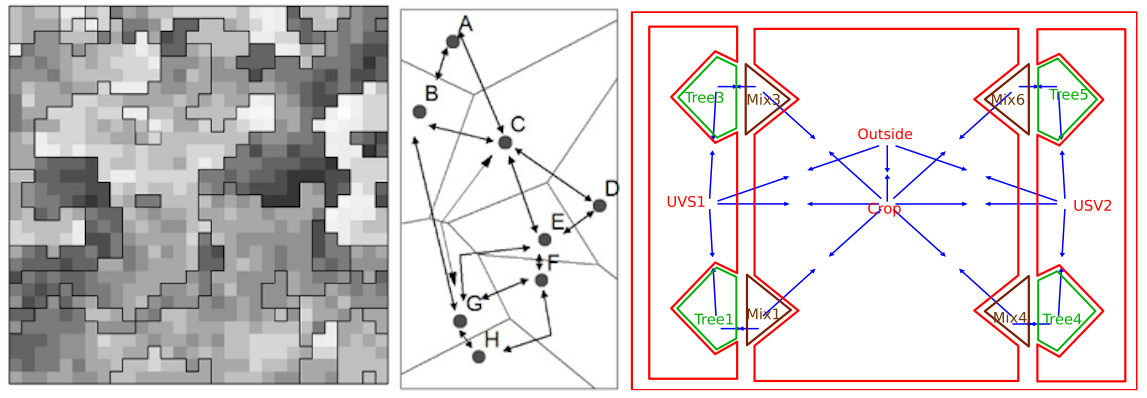
\includegraphics[width=.8\linewidth]{grid-based-modeling-teaser.png}
\caption{Site-based models partition the environment into discrete regions with locally uniform properties. Examples include (left) regular grids, (middle) Voronoi cells, and (right) generalised topological maps \cite{Nelson2012,Lemiere2023}.}
\label{fig:env-obj-grid-based-models}
\end{figure}

Site-based models represent the environment as discrete regions with uniform properties, interacting primarily with their immediate neighbours (\cref{fig:env-obj-grid-based-models}). The concept generalises to other tessellations such as Voronoi diagrams or arbitrary graphs.

\subsubsubsection{Grid-based models}

Grid-based models represent ecosystems by discretising continuous space into a regular arrangement of cells, typically squares or rectangles, each containing uniform environmental properties and ecological conditions (\cref{fig:env-obj-grid-based-models}, left). In this approach, each cell represents a spatially explicit patch hosting one or multiple populations, with interactions primarily occurring between neighbouring cells. The central ecological rationale for employing grid-based models is their conceptual simplicity, computational efficiency, and ease of representing spatial processes such as diffusion, dispersal, competition, or predation.

Mathematically, grid-based ecological dynamics are commonly described using discrete-time state equations that represent how the state of a cell (e.g., population density, biomass, or nutrient availability) changes according to its local interactions. A general formulation of these dynamics can be expressed as:
\begin{align}
N_{t+1}(x,y) = f(N_t(x,y), \Bar{N}(x, y), E_t(x, y))
\end{align}
where $N_t(x, y)$ is the state variable at cell coordinates $(x, y)$ at time $t$, $\Bar{N}(x, y)$ is the neighbourhood of the cell at coordinates $(x, y)$, $E_t(x, y)$ is the explicit environmental factors (e.g., precipitation and soil nutrients), and $f$ is the update function that describes the biological changes given the current state, the neighbourhood and the environmental factors around a cell.

Grid-based models are particularly suited for simulations involving diffusion-like processes or phenomena with clear spatial boundaries. Classic examples in ecology include modelling vegetation dynamics in arid ecosystems, spatially explicit predator-prey interactions, forest-fire spread, and habitat fragmentation effects. Additionally, grid-based representations form the basis for Cellular Automata models, where cells exhibit discrete states (e.g., occupied, empty, burning), updated synchronously according to predefined state-transition rules.

Grid-based models are commonly used due to computational simplicity, easy integration with geographic information systems (GIS), and suitability for parallel computing. They facilitate large-scale ecological modelling by clearly defining spatial relationships and boundary conditions, thus making them practical for exploring broad-scale ecological hypotheses or management scenarios.

However, significant limitations exist, as ecological processes may differ drastically at varying scales (e.g., local vs. landscape-level processes). Incorrect spatial resolution of the grid cells can lead to ecological inaccuracies or oversimplifications. Moreover, grid cells assume ecological homogeneity within each cell, which may poorly reflect natural ecological heterogeneity, especially in large cells. Complex ecological interactions, such as asymmetric competition or directional effects, are typically simplified or lost in grid-based discretisation. Finally, regular grids impose artificial directional biases (e.g., horizontal/vertical) that can impact ecological interpretations, especially for processes that depend on continuous spatial gradients or isotropy.

\subsubsubsection{Tessellation models}

Tessellation models generalise the idea of grid-based approaches by partitioning continuous ecological space into discrete regions based on proximity rather than regular shapes (\cref{fig:env-obj-grid-based-models}, centre). Among these methods, Voronoi diagrams (also known as Thiessen polygons in ecological studies) and their dual, Delaunay triangulations, are particularly relevant and widely applied.

Voronoi diagrams partition a plane based on a set of points (e.g., tree positions, animal territories, or resource centres). Each region in a Voronoi diagram is defined as the set of all points closer to a specific focal point (seed) than to any other point. Formally, given a set of points ${p_1, p_2, ..., p_n}$, the Voronoi region $V_i$ associated with the point $p_i$ is defined as:
\begin{align}
V_i = { x \in \R^2 : d(x, p_i) \leq d(x, p_j), \forall j \neq i }
\end{align}
with $d(x, p_i)$ the distance between the point $x$ and the seed $p_i$.

Conversely, the Delaunay triangulation is the dual graph structure of a Voronoi diagram. It connects points whose Voronoi regions share a common boundary, thereby explicitly defining neighbourhoods among entities (e.g., individuals or resource patches). This duality between Voronoi and Delaunay representations provides two complementary perspectives: territorial partitioning (Voronoi) and direct adjacency or connectivity (Delaunay).

In ecological modelling, these tessellation methods have significant implications and applications. Voronoi diagrams naturally represent resource partitioning among individuals or populations, capturing territorial or competitive interactions without the artificial constraints imposed by fixed grids \cite{Castle2006}. For instance, they have been effectively employed in forest ecology to model individual-tree resource competition, where the area of a tree's Voronoi cell directly correlates to available resources and competitive interactions.

The use of tessellated models may become very useful as they adapt to irregular spatial distributions, accurately modelling ecological territories and resource accessibility based on actual entity locations.

They inherently define spatial neighbourhoods without arbitrary distances or predefined shapes, enabling more precise representation of interactions among entities.

Unlike grids, Voronoi cells automatically adjust spatial resolution according to entity density, allowing finer resolution in densely populated areas and coarser resolution in sparse ones.

However, Voronoi-Delaunay models also present several limitations and challenges:
\begin{Itemize}
\Item{} Dynamic updating of Voronoi diagrams and Delaunay triangulations is computationally more intensive than fixed-grid models, especially in large-scale or highly dynamic ecosystems where individuals frequently appear, disappear, or move.
\Item{} Voronoi models implicitly assume isotropic interactions (competition or resource usage is equal in all directions) and strictly distance-based territories, neglecting directional biases such as prevailing winds, slopes, or anisotropic resource gradients.
\end{Itemize}


Generalised topological maps represent ecosystems using abstract spatial relationships and connectivity structures, emphasising the importance of spatial relationships or interactions rather than explicit geometric positions or shapes \cite{Urban2009}. Unlike grid-based or Voronoi-Delaunay tessellation models, generalised topological maps prioritise topological relationships over exact geometric distances or spatial coordinates (\cref{fig:env-obj-grid-based-models}, right). Formally, these maps can be defined as graphs or networks $G = (V, E)$, where vertices $V$ represent spatial entities (e.g., habitat patches, resources, individuals, or territories), and edges $E$ define ecological interactions, such as connectivity, dispersal pathways, competitive influence, or predator-prey relations \cite{Hamonic2021,Minor2008,Peterson2024}.

By abstracting space into relational networks, these maps enable efficient representation and analysis of ecological processes in scenarios where exact geometry may be unknown, less relevant, or overly complex. They are particularly valuable in modelling metapopulation dynamics, habitat connectivity, or animal movement patterns, where the critical ecological factor is the presence or absence of connectivity rather than explicit spatial positions. Furthermore, generalised topological approaches facilitate integration with network theory, providing tools to analyse ecological resilience, robustness, fragmentation, and connectivity dynamics directly through graph-based metrics (e.g., connectivity indices, centrality measures, or modularity analyses) \cite{Lemiere2023,Gaucherel2012}.

However, the use of generalised topological maps also presents several limitations and ecological assumptions:
\begin{Itemize}
\Item{} Removing explicit geometry sacrifices detailed spatial realism, potentially limiting the ability to accurately model distance-dependent ecological processes such as diffusion or continuous dispersal.
\Item{} Ecological outcomes can be highly sensitive to how vertices and edges are defined, necessitating careful selection or validation of the underlying graph structure to avoid artificial ecological patterns or biased results.
\Item{} Empirical calibration or validation may be difficult, as topological maps represent abstract ecological relationships rather than measurable spatial distances or tangible boundaries.
\end{Itemize}

Despite these limitations, generalised topological maps remain valuable tools, especially when combined with explicit spatial approaches \cite{Ecormier-Nocca2021} or when explicit geometry is unavailable or unneeded \cite{Duflot2018,Boussange2022}.

\subsubsection{Individual-based models}

\begin{figure}[H]
\centering
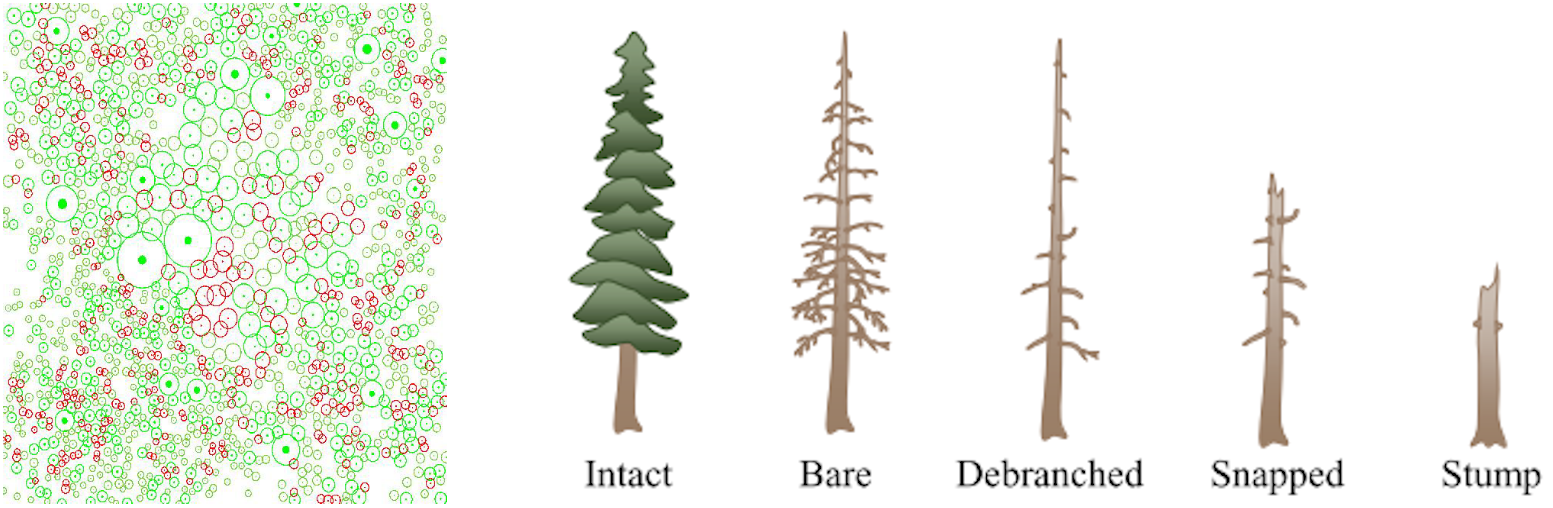
\includegraphics[]{individual-based-modeling-teaser.png}
\caption{Individual-based models focus attention on each element of the scene, with interaction between neighbouring entities. This perspective allows for more precision on (left) the positioning of each tree \cite{Alsweis2006}, but also on (right) the life cycle and geometry of the individuals \cite{Peytavie2024a}.}
\label{fig:env-obj-individual-based-models}
\end{figure}

In contrast to aggregated or spatially discrete models, Individual-Based Models (IBMs) explicitly represent each organism or ecological entity as a distinct unit \cite{Crooks2017}. Thanks to increased computational power, IBMs have gained popularity due to their ability to capture individual variability, spatial heterogeneity, and detailed ecological dynamics. In IBMs, each organism is modelled independently, enabling fine-grained representation of processes such as birth, growth, reproduction, mortality, dispersal, and competition, each potentially influenced by local environmental conditions or interactions with neighbouring individuals \cite{Chng2013,Peytavie2024a}.

IBMs inherently capture the variability and heterogeneity of natural ecosystems, thus providing ecological realism by explicitly modelling individual variability in life histories, behaviour, and spatial positioning \cite{McLane2011,Zhang2020}. As such, IBMs are particularly effective for simulating complex ecological processes, including species interactions, competition, predation, dispersal, and responses to spatially heterogeneous environments (\cref{fig:env-obj-individual-based-models}, right).

To reduce computational costs while maintaining ecological realism, IBMs frequently employ approximations distance-based competition methods (e.g., FRN, ZOI, FON) or stochastic processes capturing probabilistic interactions among individuals. Moreover, recent advances have improved the scalability and realism of IBMs by leveraging parallel computing and GPU-based simulations, facilitating large-scale applications.

Hybrid approaches are also common, combining IBMs with grid-based or tessellation models to balance computational efficiency and ecological detail. Such hybrids may represent environmental conditions through spatial grids or tessellations (Voronoi diagrams), while explicitly modelling organism-level behaviours and interactions individually \cite{Chng2011a}.

\subsubsubsection{Fixed-Radius Neighbourhood}

In the Fixed-Radius Neighbourhood (FRN) method, the first appearance of a distance-based method, each tree has a radius inside which we consider that there is shade and competition for nutrients. If two trees' radii intersect, a competition allows the stronger tree to survive while the weaker one dies (\cref{fig:env-obj-individual-based-models}, left).

\AltTextImage{

The computer graphics community represents the FRN constraint using Poisson Disk Sampling (\cref{fig:env-obj-poisson-example}) or blue noise approximations \cite{Deussen2000} to generate entities as points that do not fall within another entity's radius. The algorithm can be accelerated using a regular grid structure as proposed by \citep{Bridson2007b}: each cell of the grid has a width of $\frac{\radius}{\sqrt{n}}$ with $n$ the number of dimensions (usually $n = 2$). Each point sampled is encoded by the grid cell in which it resides. A cell can only contain a unique point, making it a fast spatial structure for distance computation with other points. Each point added to the grid recursively instantiates new random samples in a spherical annulus between radius $\radius$ and $2\radius$. While this method is fast and simple, other methods propose variations to guarantee maximal coverage \cite{Ebeida2011} or GPU parallelisation \cite{Wei2008}. However, in the presence of at least two species with different radii, the circle packing problem becomes more complicated and requires a larger number of collision checks, while still relying on the spatial indexing method from Bridson's algorithm.

}{Poisson_disk_sampling.png}{Poisson Disk Sampling iteratively adds points in space and checks whether new points fall inside the radius of previously instantiated ones.}{fig:env-obj-poisson-example}

\AltTextImage{
\subsubsubsection{Zone of Influence}
The Zone of Influence (ZOI) model is an ecological method designed to quantify competition among trees by modelling their interactions as gradual rather than binary processes \cite{Czaran1998}. In contrast to a simple binary approache proposed with Fixed-Radius Neighbourhood, the ZOI model assigns each tree a circular influence zone, typically defined based on measurable attributes such as diameter at breast height (DBH), crown dimensions, or species-specific ecological characteristics.

In this framework, competition between adjacent trees is quantified by calculating the fractional overlap between their influence zones (visible in \cref{fig:env-obj-zoi-scheme}). 

}{ZOI-Peters2020.png}{ZOI is represented by regions around entities. The intersection between two circular regions (radii) defines the competition between the two entities. Top: Symmetric competition (equal resource sharing, with the competition at the intersection divided equally); bottom: Asymmetric competition (larger entity captures more resources, such as light).}{fig:env-obj-zoi-scheme}

Mathematically, the intensity of competition $C_{ij}$ exerted by a neighbouring tree $j$ on a focal tree $i$ is expressed as:
\begin{align}
C_{ij} = \frac{ \Area_{\text{overlap}, ij} }{ \Area_{\text{ZOI}, i} }
\end{align}
where $\Area_{\text{overlap}, ij}$ is the area of overlap between the radii of trees $i$ and $j$, and $\Area_{\text{ZOI}, i}$ is the total area of the influence zone of tree $i$. This intersection area can be computed directly with:
\begin{align}
\Area_{\text{overlap}, ij} = &r_i^2 \cos^{-1}\left( \frac{d^2 + r_i^2 - r_j^2}{2 d r_i} \right) + r_j^2 \cos^{-1} \left(\frac{d^2 + r_j^2 - r_i^2}{2 d r_j} \right) \nonumber \\
& - \frac{1}{2} \sqrt{(-d + r_i + r_j)(d + r_i - r_j)(d - r_i + r_j)(d + r_i + r_j)}
\end{align}
assuming $r_i$ and $r_j$ are the radii of trees $i$ and $j$ respectively, and $d$ the distance between the two centres.

The biological consequences of competition quantified by ZOI, such as reduced growth or increased mortality risk, can be represented through growth-response equations. For instance, tree growth under competition might be modelled as \cite{Das2012,Uriarte2004}:
\begin{align}
G_i = G_{\text{max}, i} \left(1 - \alpha \sum_{j} {C_{ij}} \right)
\end{align}
with $G_i$ the growth of the tree, $G_{\text{max}, i}$ the maximal potential growth if no competition affects it, and $\alpha$ a sensitivity parameter determining how competition impacts growth.

\AltTextImage{
The ZOI model typically assumes symmetric (isotropic) competition, meaning all trees compete equally in every direction, and the competition effect between two trees is reciprocal if their zones and dimensions are similar. However, ecological realism can be increased by adopting an asymmetric (anisotropic) version of the model, which acknowledges that competition is often directionally biased or size-dependent (\cref{fig:env-obj-zoi-scheme}). For asymmetric competition, the equation is modified by introducing weighting based on differences in tree size or dominance, for example:
}{FON-asymmetric-field-Peters2020-s.png}{A limitation of individual-based models is that the influence of each entity is often assumed to be isotropic, ignoring environmental factors. Left: competition in ZOI models is identical for each entity; right: a flow direction (black arrows) induce a deformed competition for resources. Asymmetric interaction area is much more complex to compute. }{fig:env-obj-fon-asymmetric-scheme}

\begin{align}
C_{ij} = \frac{ \Area_{\text{overlap}, ij} }{ \Area_{\text{ZOI}, i} } f(DBH_i, DBH_j)
\end{align}
with $f(DBH_i, DBH_j)$ a function that introduces asymmetry due to differences in diameter at breast height (DBH), modelling stronger resource capture by larger trees, or using $f(h_i, h_j)$ to model light competition between trees of different heights.

The ZOI model is theoretically rooted in the understanding that trees compete gradually and continuously, rather than abruptly. However, it does rely on simplifying assumptions (circular, isotropic zones, homogeneous environmental conditions, and static radii within measurement intervals) which can limit its applicability to ecological scenarios involving directional resource gradients or heterogeneous environments (\cref{fig:env-obj-fon-asymmetric-scheme}).

Empirical studies across diverse forest ecosystems have demonstrated that the ZOI approach significantly improves predictions of tree growth, survival, and mortality compared to simpler binary models such as FRN. The nuanced representation of competition offered by ZOI models better captures complex ecological dynamics, particularly in mixed-species stands, uneven-aged forests, or structurally diverse ecosystems.

\AltTextImage{
\subsubsubsection{Field of Neighbourhood}
The Field of Neighbourhood (FON) approach provides an alternative method to quantify tree competition by explicitly incorporating distance-dependent and size-dependent effects of neighbouring trees on a focal tree's growth or survival \cite{Berger2000}. Unlike the ZOI model, which uses circular zones and geometric overlaps, FON models typically rely on explicit indices that incorporate both the distance and the relative sizes of neighbouring trees, without necessarily defining explicit geometric overlap areas.

In the FON approach, competition intensity affecting a given focal tree is calculated by summing the competitive effects of neighbouring trees, typically as a weighted function of their size and distance (\cref{fig:env-obj-fon-scheme}). 
}{FON-Peters2020.png}{The FON model proposes a smoother version of the ZOI, where the intersection between two radii also accounts for the distance from the tree trunk.}{fig:env-obj-fon-scheme}

\AltTextImage{
A commonly used formulation of competition intensity $FON_i$ for a tree $i$ at distance $r$ from the trunk is expressed as
\begin{align}
FON_i(r) = \begin{dcases}
1 & \text{for } 0 \leq r < \text{RBH}, \\
e^{-\curve(r - \text{RBH})} & \text{for } \text{RBH} \leq r \leq R, \\
0 & \text{otherwise}
\end{dcases}
\end{align}
with RBH the radius at breast height (half of the DBH), $R$ the radius of influence of the tree (usually proposed as $R = a \sqrt{\text{RBH}}$ with a scaling parameter $a$), and $\curve$ an attenuation coefficient, defined for each species.
}{DBH-measure.png}{DBH (and RBH) is measured at 1.3 m above ground level.}{fig:env-obj-dbh}

\AltTextImage{
The overall competition at any point in space can now be described as:
\begin{align}
F(x, y) = \sum_{i} {FON_i(x, y)}
\end{align}
The competition perceived by a tree $i$ is the average of all $FON$ values around its area $A$ (denoting $A' = \Area_{\text{overlap}, ij}$):
\begin{align}
    F_A^i = \frac{1}{A} \sum_{j \neq i}{ \int_{A'}{FON_j(x, y) \, da'} }
\end{align}
}{FON-scheme-Berger2000.png}{The evaluation of the FON value at any point is done by accumulating all individual fields.}{fig:env-obj-fon-compute-scheme}

Unlike the ZOI method, the FON model does not assume a hard boundary around each tree, instead explicitly capturing a smooth decline in competitive impact with increasing distance. It also inherently accommodates asymmetric competition, since larger and closer neighbours exert disproportionately stronger competitive influences than smaller or more distant trees (\cref{fig:env-obj-fon-compute-scheme}).

The FON method does not rely explicitly on geometric overlap and is thus flexible and particularly useful in heterogeneous forests. However, to capture the self-thinning property of silviculture \cite{Makowski2019}, satisfying $W = \curve N^{-\frac{3}{2}}$ (with $W$ the average biomass of an individual, $N$ the density, and $\curve$ a constant) \cite{Westoby1984}, the generation of the ecosystem should be iteratively simulated with small time steps \cite{Alsweis2005}, which is computationally expensive. Rather than simulating the full growth model of vegetation, most ecosystem generation algorithms focus on the distribution of the elements of the terrain, abstracting the competition into distance function deformations or statistical optimisation.

\AltTextImage{
By designing non-monotonic field functions around trees, emergent behaviours can appear. \cite{Lane2002} proposed to apply a "deformation kernel" on the distance function, resulting in a larger variety of patterns, such as the clustering of bushes and the competition of larger trees (\cref{fig:env-obj-kernels-Lane2002}, top left). Building on this idea, defining deformation kernels for each pair of species (\cref{fig:env-obj-kernels-Lane2002}, top right, with kernels for two species) allows the system to include ecological interactions between different species in the terrain. As a result, the simulation can introduce intra-species clumping while maintaining inter-species segregation.
}{kernel-matrices-Lane2002.png}{The deformation of neighbourhood kernels enables modelling of different behaviours for species and their interactions. Top-left: different kernels generate different layouts; Top-right: a matrix $M$ encodes a distance kernel for each pair of species; Bottom: using a single matrix provides a way to control the interaction of two species in a scene.}{fig:env-obj-kernels-Lane2002}

\AltTextImage{
    Alternatively, learning the spatial distribution of distances between individuals from examples can be used as a statistical metric to introduce interactive tools for ecosystem generation \citep{Emilien2015a} (\cref{fig:env-obj-worldbrush-Emilien2015}). In this work, given a user-provided example, the system learns parameters such as the histogram of inter- and intra-species distances from one region and reproduces these distributions in another region. This method is not limited to vegetation, but may include any scene elements (e.g., houses and roads), and can integrate other metrics such as terrain slope.
}{worldbrush-Emilien2015.png}{Using statistical distribution from an input terrain, \cite{Emilien2015a} synthesise a different terrain with similar distributions. Two examples are given (delimited by blue rectangular boundaries): uniform distribution (top) and clustered distribution (bottom). Differences in distribution arise from the voids in the regions of interest.}{fig:env-obj-worldbrush-Emilien2015}

While the FON model provides a biologically detailed representation of competition, its computational complexity makes it significantly more challenging to implement in large-scale simulations. Unlike the ZOI model, which relies on predefined geometric overlaps that can be calculated efficiently, the FON approach requires integrating a continuously decaying competition function over an arbitrary area of influence. This necessitates evaluating the function at multiple points across overlapping zones, increasing computational demand. Moreover, the additive nature of FON, where each tree contributes to the total competition field at every spatial point, further exacerbates the cost, scaling poorly in dense forest stands. The necessity of numerical integration or spatial discretisation makes FON computationally expensive compared to ZOI, which only requires simple geometric calculations. Consequently, while FON is useful for small-scale or highly detailed ecological studies, it is generally impractical for large-scale forest simulations.

\subsubsection{Ecological Field Models}

\begin{figure}[H]
    \centering
    \autofitgraphics[width = .8\linewidth]{ecological-fields-example-shade-Wu1985.png, ecological-fields-example-water-Wu1985.png, ecological-fields-example-nutrients-Wu1985.png}
    \caption{Ecological Field Models represent the environment as a mathematical function where environmental properties such as humidity, shade, and nutrients are seen as distinct fields (in the figure, respectively from left to right) created by the presence of trees, bushes, and flowers.}
    \label{fig:env-obj-ecological-field-models}
\end{figure}

Modelling ecosystems requires a careful balance between biological realism and computational efficiency, especially when simulating large-scale environments. Traditional ecological models fall into two primary categories: Site-Based Models and Individual-Based Models, each with distinct advantages and limitations.

Site-Based Models discretise the environment into discrete regions, making them efficient for large-scale simulations but limited in their ability to represent smooth, continuous interactions. On the other hand, Individual-Based Models explicitly simulate each organism as an independent entity, allowing for detailed biological behaviour and interactions, but quickly becoming computationally expensive when dealing with large populations.

While these approaches have been successfully used in various ecological studies, many real-world ecological processes do not fit neatly into a discrete grid or a set of independent agents. Instead, they operate in a continuous spatial domain, where organisms interact with smooth environmental gradients rather than discrete neighbours. For example, competition for light and nutrients is not limited to direct neighbours.

To address these challenges, Ecological Field Models (EFMs) provide an alternative framework where environmental properties are represented as continuous, spatially explicit fields \cite{Wu1985}. Rather than defining interactions through direct contact (as in IBMs) or discrete adjacency (as in SBMs), EFMs describe how organisms modify and respond to smooth environmental gradients \cite{Chng2011b,Seidl2012}.

From a computer graphics perspective, EFMs share similarities with techniques used in Signed Distance Fields (SDFs). Just as SDFs encode geometric influence in a continuous field, EFMs encode ecological influence, allowing for more realistic ecosystem simulations.

EFMs are based on the fundamental idea that organisms are not isolated agents but rather integral components of their environment, influencing and being influenced by it in a spatially explicit manner (\cref{fig:env-obj-ecological-field-models} shows the effect of multiple vegetation entities on the humidity, shade, and nutrient fields of the environment). The core ecological principles behind EFMs include two key points:
\begin{Itemize}
    \Item{Continuous organism-environment interactions:} Organisms modify their surroundings in ways that extend beyond their immediate location. Environmental factors such as soil nutrients, water availability, light exposure, and chemical signals influence other species gradually across space.
    \Item{Environmental feedback:} Species respond to spatially varying gradients rather than direct neighbour-based interactions, as seen in phototropism (guiding growth toward light) \cite{Pirk2012} or root development towards nutrient-rich soils \cite{Li2023}.
\end{Itemize}

The combination of these two principles creates natural feedback loops that are explicitly modelled, allowing a more realistic representation of ecological interactions compared to static environmental assumptions in traditional models.

EFMs provide a continuous representation of environmental factors, bridging the gap between grid-based and individual-based models by modelling smooth ecological gradients, instead of forcing interactions into discrete cells. This method allows organisms to influence and respond to fields dynamically, while providing a scalable framework that avoids the computational explosion of tracking every individual separately.

While EFMs provide a biologically grounded approach to modelling spatial interactions, their implementation requires a robust mathematical framework to define how organisms modify and respond to environmental fields.





An ecological field represents a spatially varying environmental property across a landscape. Mathematically, we can define an $n$-dimensional ecological field as a scalar field:
\begin{align}
F(\p) : \R^n \to \R
\end{align}

Any organism in the scene has an influence on the ecological fields through "influence functions" $K$. These functions describe how an organism's presence affects its surroundings. We can then evaluate the ecological field with $N$ entities:
\begin{align}
\label{eq:env-obj-eco-field-computation}
F(\p) = F_0(\p) + \sum_{i=0}^{N}{K_i(\p)}
\end{align}
with $F_0(\p)$ the baseline environmental state.

The primary challenge in computer graphics is how to efficiently store, sample, and modify continuous environmental fields. Since EFMs define spatially varying properties, they require a structured representation that balances accuracy, efficiency, and scalability.

Several methods exist for implementing spatially explicit fields in graphics:
\begin{Itemize}
    \Item{} A common approach is to discretise the environment into a regular 2D or 3D grid, where each cell stores a value corresponding to an ecological property (e.g., soil moisture, nutrient concentration, or shading intensity). This approach has the advantage of efficient lookup and updates, and GPU compatibility at the cost of memory usage and precision loss.

    \Item{} Rather than storing explicit values at discrete locations, ecological fields can be defined using procedural functions that are evaluated dynamically. This approach is particularly relevant in procedural terrain and vegetation generation, where continuous field functions determine environmental parameters. A Signed Distance Field (SDF), frequently used in raymarching and volumetric rendering, can be adapted for EFMs by encoding environmental influence functions. This approach enables a theoretically infinite precision for a compact memory footprint at the expense of high computational demand.
\end{Itemize}

\subsubsubsection{Environmental Objects}

\begin{figure}[H]
\centering
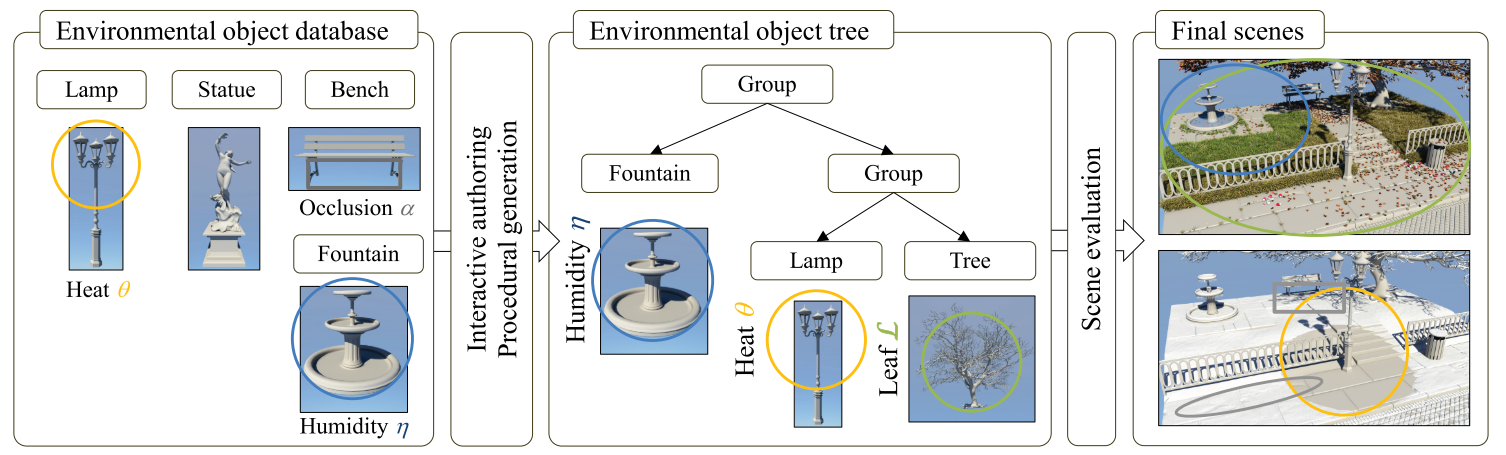
\includegraphics[]{env-objs-Grosbellet2016.png}
\caption{The Environmental Objects framework \cite{Grosbellet2016} presents a practical methodology for integrating spatially explicit environmental interactions into procedural modelling. The Environmental Objects concept aligns closely with EFMs, providing a computationally feasible way to embed field interactions into simulated ecosystems.}
\label{fig:env-obj-teaser-grosbellet2016}
\end{figure}

The Environmental Objects system of \citep{Grosbellet2016} attaches scalar fields (heat, humidity, occlusion, ...) to scene assets so that snow, leaves or soot accumulate plausibly. Although conceived for urban set dressing, the idea is strikingly similar to EFMs: objects emit and sense continuous fields and update geometry accordingly.

Our work adopts the same "fields-attached-to-objects" view but turns it into a bi-directional simulator: objects do not only read fields to change appearance, they also decide where and whether they should exist, creating an emergent distribution of terrain features.

The Environmental Objects' method presents a hierarchical framework for authoring procedural scenes by extending objects (assets) with environmental fields that control their appearance and interaction with the virtual environment (\cref{fig:env-obj-teaser-grosbellet2016}). This work tackles the main problem with modelling an urban scene, which is finding a balance between generating and editing a large scene in interactive time and the integration of small-scale details in coherence with the global environment:
\begin{Itemize}
    \Item{} Objects in a virtual scene dynamically adjust their appearance based on surrounding scalar fields, allowing for realistic procedural effects illustrated with snow deposition, leaf accumulation, and icicle formation. Unlike global simulations, which are computationally demanding, this model uses local environmental fields to procedurally generate details without requiring extensive physics-based calculations.

    \Item{} Users can modify environmental parameters, such as temperature fields, to influence scene aesthetics in an intuitive and predictable manner. The model enables scene composition through level of details using object groupings, optimising the computation of large-scale environments while maintaining local control over environmental interactions.
\end{Itemize}
By employing skeletal implicit primitives and procedural blending techniques, the framework enables the efficient simulation of environmental changes while allowing for real-time scene modifications.

In this method, each 3D model can be associated with "procedural effects", which regroup scalar fields representing changes in the environment. These fields are defined using skeleton-based implicit primitives, allowing the environment properties to be changed along a path instead of only using points like the initial EFM. This enables the system to represent, for example, the diffusion of heat around a pipe, which is not possible with the latter. The computation of an environment property is then an agglomeration of all the scalar fields associated with the given property. The authors propose computing all scalar fields, such as the heat field $\theta$, at any position $\p$ by the accumulation of objects' fields, in a similar manner as \cref{eq:env-obj-eco-field-computation}:

\begin{align}
    \theta(\p) = \theta_0(\p) + \sum_{i=1}^{n}{ \theta_i(\p)}
\end{align}

and the occlusion field $\alpha$ as the product of all objects' occlusion fields:

\begin{align}
    \alpha(\p) = \alpha_0(\p) \prod_{i=1}^{n}{\alpha_i(\p)}
\end{align}
assuming $\theta_0$ and $\alpha_0$ to be global scalar fields for temperature and shade, symbolising the baseline environmental state in the ecological domain.

\AltTextImage{
    Using the field values, the system instantiates small details such as leaves by sampling the space with candidate "anchor positions". If the field values satisfy certain conditions at the anchor position $\p_i$, the small-scale objects can be instantiated at this position (for example, for leaves: $\alpha(\p_i) l(\p_i) < d_i$ using the occlusion field $\alpha$, the leaves deposition field $l$ and the distance of the anchor position to the depositing surface $d_i$ as shown in \cref{fig:env-obj-leaves-instances}). This method can then be easily extended to modify the geometry or texture of the object based on the field values (here, the heat field and the humidity field), to manually move or rotate each of the objects, or even integrate user-defined density fields to populate entangled details on the ground \cite{Guerin2016}.
}{EnvObjs-leaves-instances-Grosbellet2016.png}{Leaves are instanced if the field values are fitted for leaves presence, and the geometry and texture are altered depending on the environment. }{fig:env-obj-leaves-instances}

\AltTextImage{
    On the other hand, the geometry of large objects can be altered using the scalar fields. The authors present a simulation of snow deposition on the objects by displacing the vertices $i$ in the direction of the normals $\vec n_i$ by an amount depending on the environment (\cref{fig:env-obj-snow-Grosbellet2016}):
    \begin{align}
        \p_i' = \p_i + \left( \alpha(\p_i) s(\p_i) g(d(\p_i)) - \theta(\p_i) \right) \vec n_i
    \end{align}
    with $s$ the "snow field", and $g$ a snow elevation function based on the distance between the original vertex and the border of the mesh.
}{EnvObjs-snow-Grosbellet2016.png}{Snow deposition is a displacement of vertices along the normals of the mesh (left), modulated by the value of fields such as occlusion (middle) and heat (right). }{fig:env-obj-snow-Grosbellet2016}

\AltTextImage{
    In addition to the EFM framework, the environmental effects from environmental objects are not limited by points geometry as the scalar functions may use a spline primitive or be extended to volume primitives (\cref{fig:env-obj-heat-field-effect}). Translated to the ecological domain, this methodology extends the EFM as the inclusion of water bodies, essential for realistic vegetation simulation, can be taken into account by considering environmental effects from rivers and lakes which are often modelled as splines and regions in 3D modelling \cite{Emilien2015,Genevaux2013,Genevaux2015}.
}{env-obj-fields-heat-Grosbellet2016.png}{The heat field produced by a pipe uses a distance function from a line instead of a single point in space.}{fig:env-obj-heat-field-effect}

The Environmental Objects method can be seen as a variant of the EFM due to their high reliance on the idea of fields and environmental effects of each element on the environment, even if the purposes of each method are opposed: one tends to model the environment properties given the elements present while the other aims at altering the geometry of a scene given the elements in the scene, regardless of their biological nature. However, the convergence of these approaches suggests possibilities for cross-disciplinary innovation. The integration of ecological dynamics into procedural modelling could lead to more adaptive virtual environments that respond realistically to environmental changes, while procedural techniques could enhance ecological simulations by improving scalability and visualisation.

The conceptual parallels between these models suggest potential areas for cross-disciplinary application. Insights from EFM could inform procedural content generation, enabling more realistic and adaptive virtual ecosystems by incorporating agent-based dynamics, ecosystem succession models, and time-dependent environmental changes. Conversely, procedural modelling techniques from computer graphics could enhance ecological simulations, improving visualisation, scalability, and user interactivity in landscape ecology and biodiversity modelling.

The original EFMs work effectively for static environmental conditions, but many real-world ecological processes involve dynamic, time-dependent changes. For instance, soil moisture depletes over time, plant growth alters shading conditions, and chemical scent trails decay. By integrating biologically inspired feedback loops, procedural generation could extend beyond static environmental effects, enabling simulations of growth, decay, and species interactions \cite{Okubo2001,Wojtek2022}. To extend Environmental Objects beyond static environmental representations, we turn to reaction-diffusion models, which provide a mathematical foundation for modelling time-dependent field interactions used in ecological simulations.





\subsection{Diffusion models}

\begin{figure}[H]
    \centering
    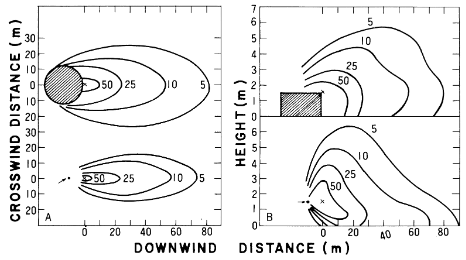
\includegraphics[]{diffusion-example-Okubo2001.png}
    \caption{The diffusion model describes the spread, motion, and evolution of a chemical, population or physical property over time. \cite{Okubo2001}.}
    \label{fig:diffusion-model-teaser}
\end{figure}

Reaction-diffusion equations, popularised by Turing \cite{Turing1952}, combine local growth/decay with spatial spread. They underpin models of vegetation patterns, invasive species fronts, or nutrient flows \cite{Cosner2008}. For our purpose they serve as analytic update rules whose steady state can be reached without time-marching every intermediate step.

Reaction-diffusion models describe the spatial and temporal evolution of populations, chemicals, or other ecological entities that interact (reaction) and spread (diffusion) through a medium (\cref{fig:diffusion-model-teaser}). These models are widely used in ecosystem simulations to understand population dynamics, species dispersal, disease spread, and spatial pattern formation in ecological systems.

In the context of ecology, a reaction-diffusion model typically represents:
\begin{Itemize}
    \Item{} Reaction: Local changes in population density due to birth, death, predation, or competition.
    \Item{} Diffusion: Movement of individuals or species across space due to random dispersal or environmental factors.
\end{Itemize}
These models help ecologists predict how populations evolve over time and across space, providing insights into species survival, biodiversity, and ecosystem stability.

The classical reaction-diffusion equation is expressed as:

\begin{align}
    \label{eq:env-obj-classic-reaction-diffusion}
    \frac{\partial u (x, t)}{\partial t} = D \nabla^2 u(x, t) + R(u)
\end{align}

where $u(x,t)$ represents the population density (or concentration of a substance) at position $x$ and at time $t$, $D$ is the diffusion coefficient, determining the rate of spatial spread. $\nabla^2 u$ is the Laplacian operator, representing diffusion across space and $R(u)$ is the reaction term, which models growth, decay, or interactions between species.

\subsubsection{Diffusion term}
Diffusion is a fundamental process in ecological modelling that describes how individuals or substances spread across space due to random movement or environmental influences. In ecosystems, diffusion can model species dispersal, nutrient transport, disease spread, and invasive species expansion.

In mathematical models, diffusion is typically represented as a term in partial differential equations that governs how population densities change over time and space. While many ecological models assume isotropic diffusion (movement occurs equally in all directions), anisotropic diffusion provides a more realistic representation of species movement in structured or heterogeneous landscapes.

However, when diffusion is anisotropic, the diffusion coefficient varies depending on direction, and we must generalise the equation (\cref{eq:env-obj-classic-reaction-diffusion}) by introducing a diffusion tensor $\tensor{D}$ \cite{Ramos2024}:

\begin{align}
    \label{eq:env-obj-reaction-diffusion}
    \frac{\partial u (x, t)}{\partial t} = \nabla \cdot (\tensor{D} \nabla u(x, t)) + R(u)
\end{align}

The tensor $\tensor{D}$ can now encompass the effect of relief and environmental factors such as wind and currents in the spread of a species. When diffusion is isotropic, $\tensor{D} = D\tensor{I}$, reducing the equation to the classic isotropic form.

Anisotropic diffusion is particularly useful in ecological modelling where movement rates are not uniform due to environmental structures or organism behaviour. For example, wind influences the spread of pollen, seeds, and insect populations, leading to anisotropic diffusion. Similarly, marine organisms or pollutants diffuse anisotropically in ocean currents.
Invasive species may spread preferentially along corridors such as rivers or roads, causing asymmetric diffusion. In ecosystems where microorganisms move in response to chemical gradients (chemotaxis), anisotropic diffusion better models movement patterns.

We may generalise the reaction-diffusion equation to account for both internal (density, species interaction, ...) and external (environmental factor, relief, seasonality, ...) influences on diffusion by slightly rewriting \cref{eq:env-obj-reaction-diffusion}:
\begin{align}
    \frac{\partial u}{\partial t} = \nabla \cdot (\tensor{D(*)} \nabla u) + R(u)
\end{align}
where $\tensor{D(*)}$  is a diffusion tensor dynamically defined by any relevant internal or external property of the system. For example:
\begin{Itemize}
    \Item{} A density-dependent diffusion can be expressed as $\tensor{D(*)} = \tensor{D} u^m$, allowing for crowding or dispersal-limited movement \cite{Zhu2023}.
    \Item{} A seasonal dispersal effect can be incorporated as $\tensor{D(*)} = \tensor{D} (1 + A cos(\omega t) )$, where dispersal varies cyclically over time \cite{Katriel2021}.
    \Item{} A spatially varying diffusion may be defined as $\tensor{D(*)} = \tensor{D} f(x)$, such as the patchy diffusion formulation used in metapopulation models \cite{Czaran1998}:
    \begin{align}
        \tensor{D(*)} = \tensor{D} \begin{dcases}
            D_1&, x \in \text{habitable patch} \\
            D_2&, x \in \text{hostile patch}
        \end{dcases}
    \end{align}
    \Item{} An anomalous diffusion such as the inclusion of Lévy flight term, incorporating random long distance jumps can be expressed as $\tensor{D(*)} = \tensor{D} u^m + \noise L(t)$ \cite{Humphries2014,Chechkin2008}.
\end{Itemize}

This generalized form enables the integration of anisotropic effects, landscape heterogeneity, and adaptive movement behaviors within reaction-diffusion models, making it highly applicable to ecological and biological systems.

\subsubsection{Reaction term}
In physics and chemistry, the reaction $R(u)$ term describes how substances are produced or consumed in a system. Some common reaction formulations include:

\begin{Itemize}
    \Item{} Linear reaction terms (exponential growth with $\lambda > 0$ or decay $\lambda < 0$) as in the radioactive decay formulation:
    $$ R(u) = \lambda u $$
    \Item{} Second-order reactions, usually found in chemical reactions between two molecules:
    $$ R(u, v) = \alpha u v$$
    \AltTextImage{
        \Item{} Turing pattern-forming systems proposed by Alan Turing to explain stripe and spot formations in animal coat patterns and chemical reactions \cite{Turing1952,Shoji2002}
        $$ R(u, v) = \begin{dcases}
            f(u, v) & \text{(Activator)} \\
            g(u, v) & \text{(Inhibitor)}
        \end{dcases}$$
    }{turing_patterns.png}{Turing patterns on animals}{fig:env-obj-turing-pattern}
\end{Itemize}

On the other hand, in ecology, the reaction term models population growth, competition, predation, and ecosystem interactions \cite{Brauer2012}. Some of the most important ecological reaction terms are:
\begin{Itemize}
    \Item{} The logistic growth, that describes a single species population growth in a limited-resource environment, is defined with a growth rate $r$ and a carrying capacity $K$ \cite{Verhulst1844}:
    $$ R(u) = r u \left( 1 - \frac{u}{K} \right)$$
    \Item{} The Lotka-Volterra competition model, that describe the trophic interactions between two or more species, for which the reaction-diffusion equations take into account each other species:
    \begin{align}
        \frac{\partial u_i}{\partial t} = r_i u_i \left( 1 - \frac{\sum_{j=1}^N a_{ij} u_j}{K_i} \right)
    \end{align}
    with $N$ representing the number of species and $a_{ij}$ the interaction coefficient (how strongly the species $u_j$ inhibit the species $u_i$). \\
    This formulation can also be rewritten in a vectorized form as the generalized Lotka-Volterra equation:
    \begin{align}
        \tensor{f} = \tensor{r} - \tensor{A} \tensor{u}
    \end{align}
    where $\tensor{f} = (f_1, f_2, ..., f_N)^\intercal$ represents the per capita growth rates of all species, $\tensor{r} = (r_1, r_2, ..., r_N)^\intercal$ is the intrinsic growth rate vector, $\tensor{u} = (u_1, u_2, ..., u_N)^\intercal$ is the species population vector and $\tensor{A}$ is the interaction matrix, with elements $a_{ij}$ describing the effect of species $j$ on species $i$.
    
    Since population growth depends on the per capita growth rate, the full population dynamics equation follows:
    \begin{align}
        \frac{\partial \tensor{u}}{\partial t} = \tensor{u} \circ \tensor{f}
    \end{align}
    where $\circ$ represents the element-wise product, ensuring that each species' growth depends on both its population size and its per capita growth rate.
\end{Itemize}


\subsubsection{Advection}
In vegetation ecosystem modelling, advection refers to the directed transport of biological or environmental variables under the influence of external forces (e.g., wind, water flow, or slope). Unlike diffusion, which describes random movement, advection introduces a preferred direction of transport, significantly influencing ecosystem dynamics \cite{Burger2020}.

Mathematically, the advection-diffusion-reaction equation (or "scalar transport equations" \cite{Baukal2000}) extends the classical reaction-diffusion model by adding a velocity field $\field{v}$ that governs directed movement:
\begin{align}
    \frac{\partial u}{\partial t} + \field{v} \cdot \nabla u = \nabla \cdot \left( \tensor{D} \nabla u \right) + R(u)
\end{align}

In physics, the transport of a property such as heat is coupled by the diffusion process, and the advection term $\field{v} \cdot \nabla u$ may be incorporated in the diffusion coefficient $\tensor{D}$ to form the "convection term". In this work we will separate the advection term and the diffusion term for clarity.

Wind is a major dispersal mechanism for many plant species, affecting seed distribution, plant competition, and biodiversity. The dispersal efficiency of seeds and pollen depends on wind velocity, turbulence, and interactions with terrain features. In flat landscapes, wind disperses seeds relatively uniformly; however, in complex terrains, wind speed and direction are influenced by topography, vegetation cover, and atmospheric conditions. Wind channelled through valleys may enhance seed deposition in lowland areas, while mountain ridges and abrupt elevation changes can create wind shadows, reducing dispersal effectiveness.

The dispersal of seeds can be modelled using an advection-diffusion equation:
\begin{align}
    \frac{\partial S}{\partial t} + \field{v} \cdot \nabla S = \nabla \cdot (\tensor{D}_s \nabla S) - \lambda S
\end{align}
with $S(x, t)$ the seed density at position $x$ and time $t$ and $\lambda$ a mortality rate due to environmental constraints or predation.

A stochastic modelling of turbulent regime could be added to the velocity field with a stochastic noise term:
\begin{align}
    \frac{\partial S}{\partial t} + (\field{v} + \sigma(x, t)) \cdot \nabla S = \nabla \cdot (\tensor{D}_s \nabla S) - \lambda S
\end{align}

On another hand, soil moisture distribution is essential for vegetation survival and ecosystem stability. The movement of water through soil is governed by surface runoff, subsurface infiltration, and capillary action, which are affected by slope, soil texture, and plant uptake rates. In hilly or mountainous regions, gravity-driven water flow dominates soil moisture distribution, creating hydrological gradients that shape vegetation structure.

The movement of soil moisture can be approximated by the Soil Moisture Velocity Equation \cite{Ogden2017}, a modified form of the Richards equation:
\begin{align}
    \frac{\partial W}{\partial t} + \field{v} \cdot \nabla W = \nabla \cdot (D_W \nabla W ) - S
\end{align}
with $W(x, t)$ the water concentration at position $x$ and time $t$, $D_W$ the water diffusion coefficient, $S$ the plant water uptake (the amount of water absorbed or transpired, mainly by the roots of vegetation \cite{Peters2020,Shanin2015}), and $\field{v} = - K g \hat z$ a simplified velocity field provided by the slope hindered by the hydraulic conductivity $K$.

Steeper slopes enhance runoff, reducing soil water retention and increasing drought susceptibility in these regions. Conversely, water accumulates in lowland areas, promoting denser vegetation and the formation of wetlands or riparian ecosystems. As a result, topography directly influences plant distribution, with drought-resistant species dominating slopes and water-demanding species thriving in valleys.

We find in the advection-reaction-diffusion equation a general way to represent a multitude of natural phenomena: from the propagation of bacteria, prey and predators, to the spread of nutrients, of water, or even of fire \cite{Hadrich2021}.

\midConclusion

In summary, the literature offers a spectrum of discrete and continuous approaches. Our method borrows the field coupling of EFMs, the sparse symbolic efficiency of Environmental Objects, and analytic steady-state solvers from reaction-diffusion theory, combining them into a multi-scale, interactive generator suited for both underwater and terrestrial scenes.









\section{Description of the method}
\label{sec:env-obj-pipeline}

In this section, we present the pipeline that underpins our method.
We first introduce the continuous environmental fields (\glosses{EnvVal}), then the discrete actors that perceive and affect those fields (\glosses{EnvObj}), before detailing how they modify the fields (\glosses{EnvModif}) and how the full pipeline orchestrates their interaction.

Our approach introduces the concept of \glosses{EnvObj}, simplified, scale-agnostic terrain features that interact with their surroundings to simulate complex ecosystem dynamics. These \glosses{EnvObj}, which can represent natural features influence (trees, rivers, rocks, ...) and are influenced by scalar fields (temperature, humidity, elevation, ...). The method is structured into three key phases: initialization, which sets up the foundational terrain elements and \glosses{EnvObj} definitions; an iterative generation process that instantiates \glosses{EnvObj} and lets them interact with their environment; and finally, an output stage that yields a sparse representation of the scene's features. This section details each phase and explains how the system dynamically adapts to user input and environmental changes.

\subsection{\Glosses{EnvVal}}
\label{sec:env-obj-communication}

In geography, and in the Ecological Field Models reviewed earlier, a "field" is a spatially continuous variable defined at every point of the domain.
It may be a scalar (elevation, temperature) or a vector (wind, current). We follow the geographic usage of "field" as a spatially continuous attribute (scalar or vector). To avoid clashing with the algebraic "field" or computer graphics jargon, we call every such quantity an \gloss{EnvVal}.

In an ecosystem simulation, each actor of the ecosystem has an impact on all other actors, which results in an exponentially growing computation effort as the number of elements of the terrain increases. Direct pairwise interaction between $n$ organisms scales as $\mathcal{O}(n^{2})$.
Instead, we adopt the standard EFM strategy: every \gloss{EnvObj} writes to local \glosses{EnvVal} through its \gloss{EnvModif}.
Each object then reads those values later, turning the global complexity into a linear complexity per simulation step and thus remaining interactive even for thousands of objects.

We bundle the currently supported fields under the unified term "environment", denoted as $\environment = (\height, \; \Water, \; \Wlevel, \; \material)$,
where $\height$ (height) and $\Wlevel$ (water level) are scalars, $\Water$ (water currents) is a 2D vector field, and $\material$ (\glosses{EnvMat}) is a vector of per-point resource stocks (sand, salt, moisture, limestone, ...).

These \glosses{EnvMat} are conceptual reservoirs used by rule sets. They need not be visualised nor stored as layered textures.

\subsection{\Glosses{EnvObj}}
\label{sec:env-obj-environmental-objects}

\begin{figure}
    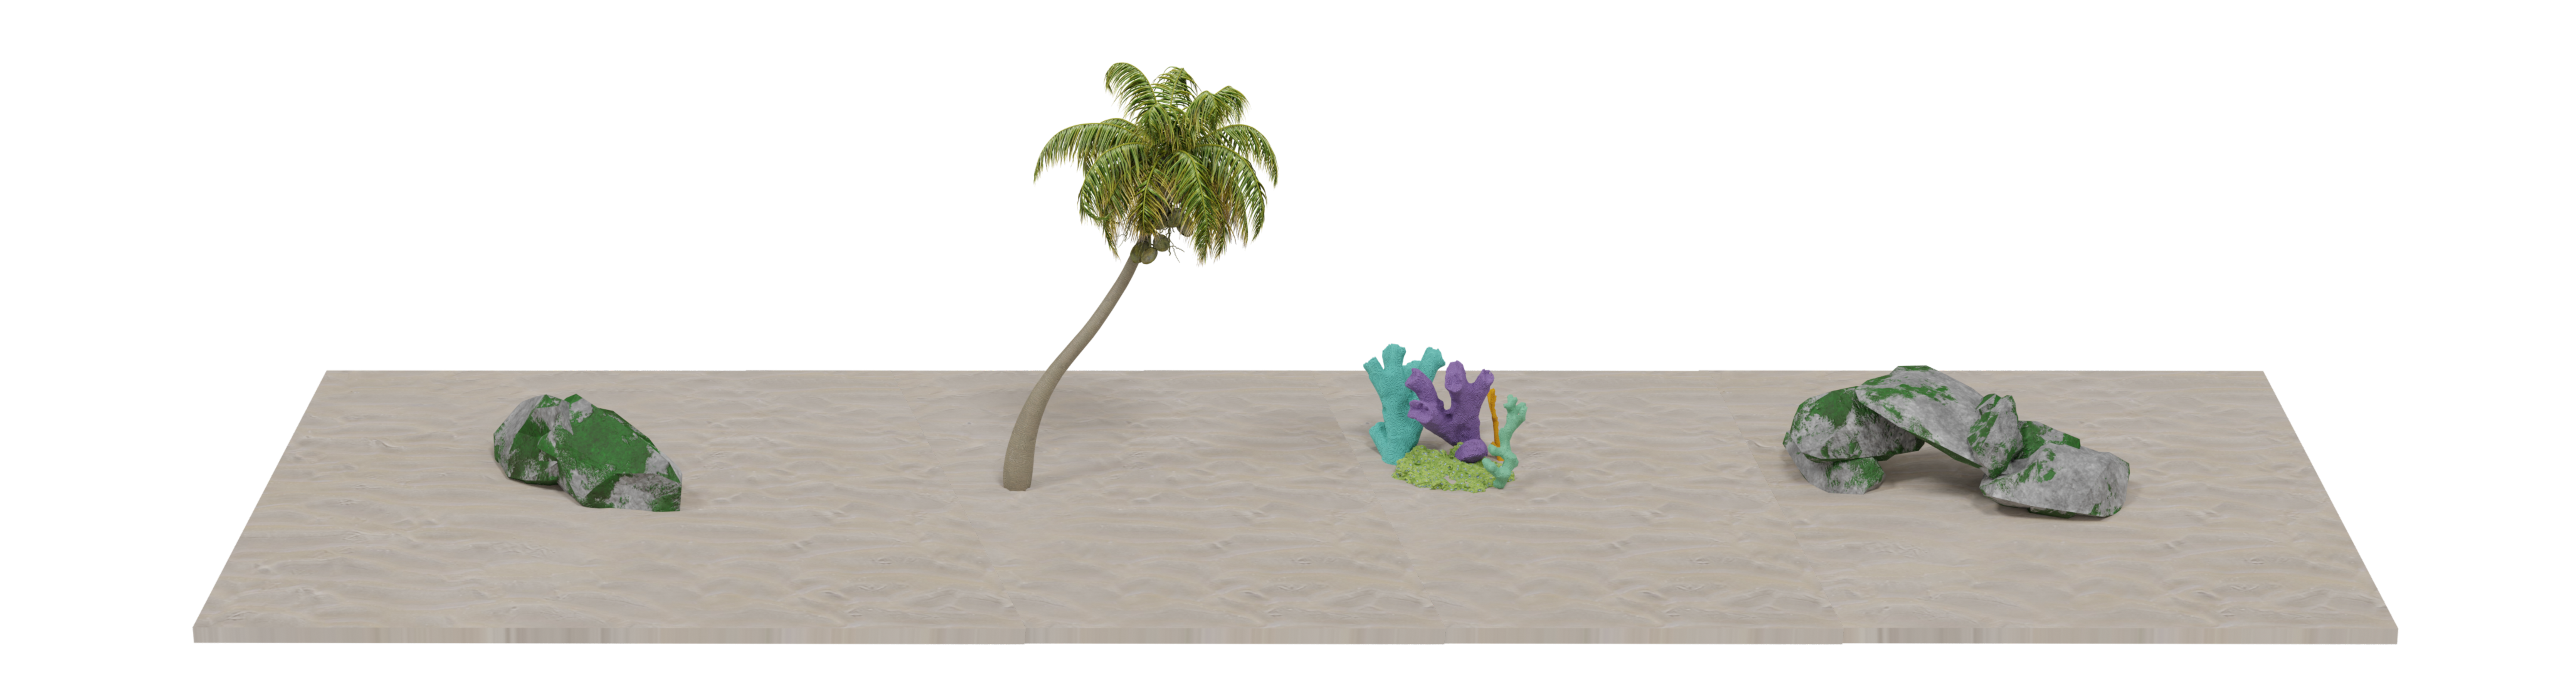
\includegraphics{assets-demo.pdf}
    \caption{\Glosses{EnvObj} can be visualised by 3D triangular meshes. From left to right: rocks, trees, corals, arches.}
    \label{fig:env-obj-assets}
\end{figure}

A geographical feature, also called object or entity, is defined as a discrete phenomenon located at or near the Earth's surface, relevant in geography and geographic information science (GIScience). It represents geographic information that can be depicted in maps, geographic information systems (GIS), and other forms of geographic media. This term includes both natural and human-made objects, ranging from tangible items (e.g., buildings or trees) to intangible concepts (e.g., neighbourhoods or savanna). Features are distinct entities with defined boundaries, differentiating them from continuous geographic masses or processes occurring over time. They can be categorised as natural features, such as ecosystems, biomes, water bodies, and landforms, or artificial features (e.g., settlements, administrative regions, and engineered constructs). As the term "feature" is overused in computer science, we will use the term \gloss{EnvObj} in this work.

\AltTextImage{
Each \gloss{EnvObj} is anchored by a skeleton (a point, curve, or region in the cartographic sense) which captures its footprint while postponing heavy geometry generation (\cref{fig:env-objs_example-scheme1}).
\begin{Itemize}
    \Item{Point-based}: isolated boulders, individual trees, individual corals, ...
    \Item{Curve-based}: river, coral reefs, fault scarps, ...
    \Item{Region-based}: islands, forests, sediment patches, ...
\end{Itemize}
}{Env-obj-scheme1.png}{Environmental objects, from 2D (top) to their 3D geometry (bottom)}{fig:env-objs_example-scheme1}

Via its prescribed \glosses{EnvModif}, an \gloss{EnvObj} locally deposits, removes, or diverts \glosses{EnvMat}, thereby updating the surrounding \glosses{EnvVal}. Conversely, its viability is re-evaluated through a user-defined \gloss{FitnessFunc} that samples those same fields. If viable, a \gloss{FittingFunc} refines the skeleton (e.g., a river streams downhill, and seagrass meadow patches are limited to luminous areas).

\subsection{\Glosses{EnvModif}}

The environment determines if a \gloss{EnvObj} belongs at a certain position.
When a \gloss{EnvObj} is placed, its surrounding \glosses{EnvVal} can be affected through \glosses{EnvModif} ($,\environmentModif = (\heightModif, \waterModif, \nothing, \materialModif),$) which define a change of height~$\heightModif$, modifications of the water current field~$\waterModif$, and \gloss{EnvMat} alterations~$\materialModif$.

\Glosses{EnvObj} are subject to altitude constraints.
However, to maintain a clear distinction between semantic modelling and 3D modelling, we do not compute the exact physical shape or detailed height field of each \gloss{EnvObj}.
Instead, we define a \gloss{CoarseHeight}~$\heightModif$, a parametric surface derived from the \gloss{Skeleton}, that provides a coarse estimate of local elevation changes. This coarse proxy lets us evaluate altitude-dependent rules without the cost of globally computing the height field.

Altering the vector field~$\Water$ is performed by composing the individual contributions $\waterModif$ of each object at position~$\p$, following \citep{Wejchert1991}. For efficiency we adopt an analytical deformation kernel inspired by Kelvinlet solutions \cite{DeGoes2017} to aggregate these local disturbances.

Each \gloss{EnvObj} possesses intrinsic \glosses{EnvMat} that both spread and are absorbed around its skeleton over time. For example, a coral colony deposits limestone while simultaneously slowing currents; the reef then uptakes that limestone for growth.
In our model the colony contributes a deposition term $\materialModif_{\text{limestone}}$, and the reef absorbs it. No direct object-object message passing is required.

Scalar \glosses{EnvVal} are updated by adding or removing mass around the \gloss{Skeleton} and then diffusing it, biased by $\Water$.
We assume a \gloss{SteadyState} regime, guaranteed by a decay rate~$\decay \in;]0; 1[$ that prevents unbounded accumulation during advection-diffusion.

\subsection{Pipeline}

\begin{figure}[H]
    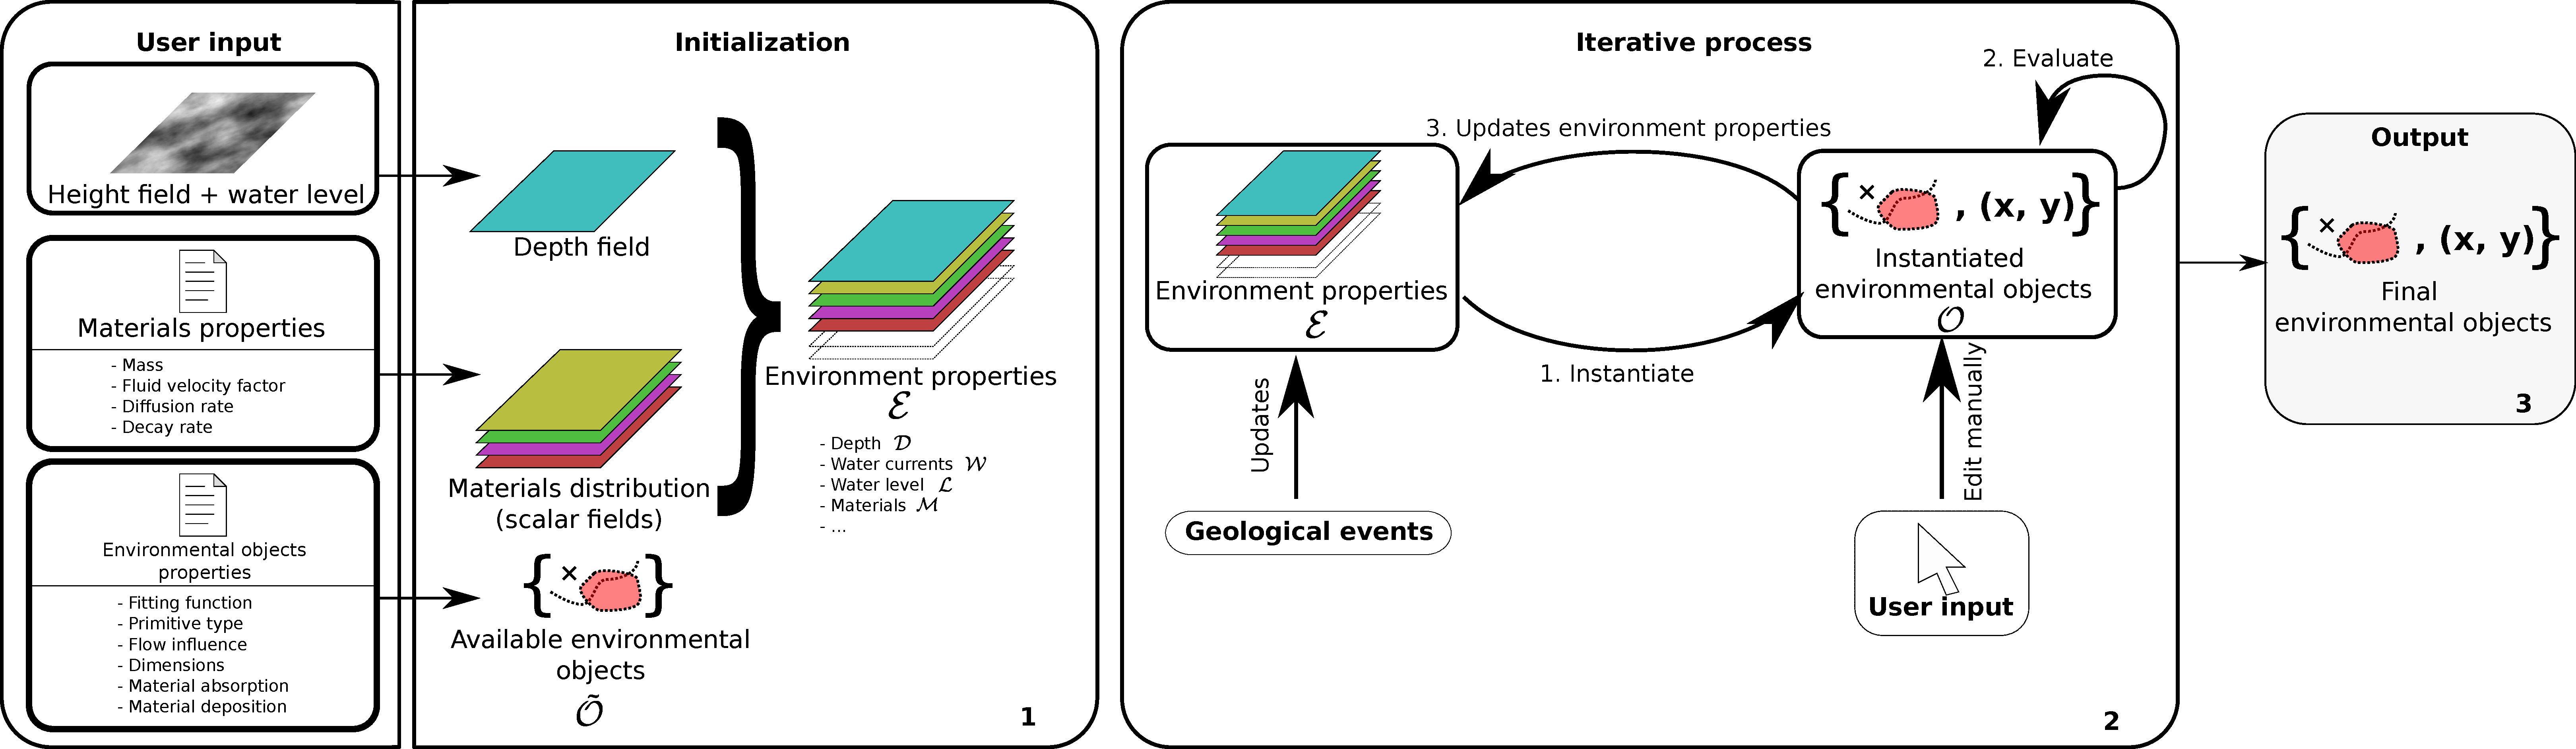
\includegraphics{pipeline.pdf}
    % \caption{Overview of the pipeline of the method: The user provides as input an initial height field and sets the water level, as well as a definition of the \glosses{EnvMat} properties and \glosses{EnvObj} properties that will be used in the iterative process. These inputs are initialised as an initial set of \glosses{EnvObj} and scalar fields that represent the \glosses{EnvVal}. In the iterative loop, new \glosses{EnvObj} are instantiated using the current state of the environment at their optimal position. The existing \glosses{EnvObj} in the terrain re-evaluate their \gloss{FitnessFunc} to grow or die and update the \glosses{EnvVal} locally. At each iteration, \glosses{GeoEvent} can update the \glosses{EnvVal}, while the user can interact directly with the \glosses{EnvObj}. The result of the whole process is a set of \glosses{EnvObj}, which is a sparse representation of the features of the scene.}

    \caption{Overview of the pipeline of the method. Three different inputs are required at initialization (left): a base terrain and a given water level directly given by the user for each generated scene, a set of properties for the \glosses{EnvMat} available (\cref{sec:env-obj-pipeline}), and the properties and generation rules of \glosses{EnvObj} available (\cref{sec:env-obj-environmental-objects}), established with experts. The generation process (middle) iteratively proceed in three steps: instantiating new \glosses{EnvObj} (\cref{sec:env-obj-generation-rules}), evaluating the fitness of each entity with respect to user modifications (\cref{sec:env-obj-interaction}), and updating the environment until stabilisation (\cref{sec:env-obj-materials}) with user-defined geomorphological events (\cref{sec:env-obj-events}). When the scene suits the user, the sparse representation of \glosses{EnvObj} in the scene is returned and can be rendered (right). }
    % The user provides as input an initial height field and sets the water level, as well as a definition of the \glosses{EnvMat} properties and \glosses{EnvObj} properties that will be used in the iterative process. These inputs are initialised as an initial set of \glosses{EnvObj} and scalar fields that represent the \glosses{EnvVal}. In the iterative loop, new \glosses{EnvObj} are instantiated using the current state of the environment at their optimal position. The existing \glosses{EnvObj} in the terrain re-evaluate their \gloss{FitnessFunc} to grow or die and update the \glosses{EnvVal} locally. At each iteration, \glosses{GeoEvent} can update the \glosses{EnvVal}, while the user can interact directly with the \glosses{EnvObj}. The result of the whole process is a set of \glosses{EnvObj}, which is a sparse representation of the features of the scene.}
    \label{fig:env-obj-pipeline}
\end{figure}

\subsubsection{Initialization}

We initialise the terrain with a height field $h$ and a water level $\Wlevel$. During this chapter we will include many \glosses{EnvObj} depending on altitude or depth, so we will use the shorthand notations $\height = h-\Wlevel$ (signed height above water) and $\depth=-\height$ (signed depth below water). The height field provides variation in altitude, which can influence the generation process of the scene.

A catalogue of available \glosses{EnvObj} $\availableObjects$ is supplied, as well as an optional target list of \glosses{EnvObj} $\targetObjects$ used as a stop condition of the process.

Finally, different \glosses{EnvMat} are defined with properties: diffusivity, density, decay rate, and advection sensitivity. These parameters are chosen with field experts to reflect plausible physical behaviour.

An initial environment configuration, resulting from the initial height field $h$ and water level $\Wlevel$, the \glosses{EnvMat} distribution $\material$ (represented as scalar fields $\material: \R^2 \to \R$), and water currents $\Water$ (as a vector field $\Water: \R^2 \to \R^2$), is then available for all \glosses{EnvObj} to evaluate growth and spawning. The \glosses{EnvVal} is noted $\environment = (\height, \Water, \Wlevel, \material)$ (\cref{sec:env-obj-communication}).

The definition of \glosses{EnvObj} properties and \glosses{EnvVal} is done with field experts, who first decide which \glosses{EnvMat} layers are relevant for the target biome and then anchor the corresponding parameters in the system.
The generation phase starts from this environment plus an optional seed set of \glosses{EnvObj}.

\subsubsection{Generation process}

After initialization, the system enters an incremental loop with two stages:
\begin{Itemize}
    \Item{-} instantiate candidate \glosses{EnvObj}, then
    \Item{-} update the environment.
\end{Itemize}
The loop terminates when user-defined criteria are met (e.g.\ an iteration count threshold, the target set of \glosses{EnvObj} $\targetObjects$, or manual approval).

\subsubsubsection{Instantiation}

Each iteration proposes new \glosses{EnvObj} at locations sampled stochastically and ranked by their \glosses{GenRule} (\cref{sec:env-obj-generation-rules}).
Every instantiated object immediately evaluates its own viability through the user-supplied \gloss{FitnessFunc} and adjusts shape and pose with the \gloss{FittingFunc}.

\subsubsubsection{Environment update}

After instantiation, every \gloss{EnvObj} applies its \glosses{EnvModif}: perturbing the flow field $\Water$ (\cref{sec:env-obj-water-currents}), and deforming the coarse height field $\height$, then depositing or absorbing \glosses{EnvMat} $\material$ (\cref{sec:env-obj-materials}) as an advection-diffusion solver relaxes \glosses{EnvMat} under current-driven transport and gravity until a local steady state is reached.

At any iteration, the user may edit individual \glosses{EnvObj} interactively (\cref{sec:env-obj-manual-interaction}) or schedule \glosses{GeoEvent}, such as storms or ground subsidence, that modify \glosses{EnvVal} globally (\cref{sec:env-obj-events}).

\subsubsection{Output}

The output of our system is a set of \glosses{EnvObj} stored as 2D skeletons in the plane. We deliberately stop at this sparse, symbolic level; meshing, texturing, and final rendering are left to downstream tools chosen by the end-user. For each object, we export its skeleton geometry, semantic class, and environment-modifier parameters, enough to drive terrain synthesis or placement of assets in a game engine or simulator. Figures in this chapter illustrate possible renderings generated with a mix of implicit surfaces and triangular meshes (\cref{fig:env-obj-assets}).

\section{Placement of \glosses{EnvObj} in an environment}
\label{sec:env-obj-generation-rules}

At each iteration of our algorithm, we aim to place new \glosses{EnvObj} at plausible locations. Because we do not enforce physical time continuity, our goal is to progressively enrich the scene according to user intent while maintaining ecological and geological plausibility.
Because each \gloss{EnvObj} modifies the environment when instantiated, potentially destabilising previous placements, the goal is to insert new elements where they minimally disturb the existing scene.

Our placement algorithm proceeds in two steps: first, it identifies the globally most suitable position using the \gloss{FitnessFunc} $\fitnessFunc: \environment \to \R$, which depends on environmental factors such as altitude $\height(\p)$, water flow $\Water(\p)$, water level $\Wlevel(\p)$, and material availability $\material(\p)$. Second, it refines the object's shape and pose using its \gloss{FittingFunc} $\fittingFunc: \environment \to \R$.

For notational simplicity, we abbreviate $\fitnessFunc(\environment(\p))$ and $\fittingFunc(\environment(\p))$ as $\fitnessFunc(\p)$ and $\fittingFunc(\p)$, respectively.

\subsection{\Gloss{FitnessFunc}}

\begin{figure}
    \autofitgraphics[]{coral-erosion-example.pdf, rock-erosion-example.pdf}
    \caption{While the \gloss{FitnessFunc} guides the position of the \glosses{EnvObj}, the \gloss{FittingFunc} provides an indication of the suitability of the \gloss{EnvObj} in its surroundings. This information is used to determine if the \gloss{EnvObj} should be removed, but may also be used for visual purposes to indicate unhealthy corals or eroded rocks.}
    \label{fig:env-obj-procedural-erosion}
\end{figure}

"Darwinian fitness" refers to an organism's ability to survive and reproduce in its environment. It is a measure of how well-suited an organism is to its surroundings, and those with higher fitness are more likely to pass on their genes to the next generation. In a similar vein, the \gloss{FitnessFunc} of a \gloss{EnvObj} evaluates its suitability at a location in the terrain, extending the meaning to living features (e.g., forests and corals) and non-living elements (e.g., rivers, mountains and karsts).

The fitness function $\fitnessFunc$ quantitatively evaluates how well a given environment location satisfies the requirements of an environment object (\gloss{EnvObj}). In other words, $\fitnessFunc$ returns a numeric score representing the suitability of local environmental conditions for that object. This function considers various environmental variables such as altitude, the presence of specific materials, water current strength, and their respective gradients. Crucially, $\fitnessFunc$ is defined separately for each \gloss{EnvObj} class, allowing it to be tailored to the unique needs and tolerances of different object types. Higher $\fitnessFunc$ values indicate more favourable sites for the object, while lower values correspond to less suitable or inhospitable locations.

Different types of \glosses{EnvObj} require different criteria for their fitness evaluation. For example, a river might prioritise lower altitude and proximity to water currents, while a forest might prioritise higher altitude and specific material availability. The flexibility of the fitness function allows it to be customised for each \gloss{EnvObj}, ensuring that the generated terrain remains coherent and realistic.

In practice, to find suitable locations for an object, we evaluate its $\fitnessFunc$ across the environment's spatial domain. This typically involves sampling $\fitnessFunc$ values on a grid or at numerous candidate points covering the area of interest, effectively producing a fitness map for that object class. If an object occupies an area (rather than being point-like), the fitness of a proposed placement can be obtained by aggregating $\fitnessFunc$ over that area by averaging the fitness values at multiple sample points within the object's footprint. The outcome is a field of fitness values where peaks indicate highly suitable locations. Each object class thus yields its own fitness landscape.

The value of the \gloss{FitnessFunc} can be used later on to modify the geometric representation or the appearance of the \gloss{EnvObj} to appear more eroded (\cref{fig:env-obj-procedural-erosion}).

\subsection{\Gloss{FittingFunc}}

A candidate object is first seeded at the point $\p_s=\arg!\max_\p \fitnessFunc(\p)$, i.e.\ the global maximum of the fitness map. This seed acts as the initial guess for the subsequent shape optimisation described below. Moreover, this two-step optimisation allows a coarse approximation of the global maximum of the \gloss{FitnessFunc} with few samples, reducing its computational demand, as the \gloss{FittingFunc} optimisation is focused on a single seed.

\subsubsection{Point-based \gloss{Skeleton}}

For objects whose skeleton reduces to a single point (boulders, solitary corals, etc.), we refine the seed by hill-climbing on a (possibly different) fitting field $\fittingFunc$. In most cases we simply set $\fittingFunc=\fitnessFunc$, but the user may supply a sharper or multi-objective field when needed. Optimisation proceeds by gradient ascent on $\nabla\fittingFunc$ with a small step size and terminates when $|\nabla \fittingFunc|<\varepsilon$.

\subsubsection{Curve-based \gloss{Skeleton}}

The skeleton of a curve-based \gloss{EnvObj} is determined by the shape that fits best given the environment it is added to.
Using an Active-Contour ("snake") formulation \cite{Kass1988}, we seek a parametric curve $\curve(s)!:![0,1]!\to!\R^{2}$ that minimises the composite energy
\begin{align}
\energy(\curve) = \Einternal + \Eexternal + \Eshape + \Egradient
\end{align}
with
\begin{align}
    \label{eq:env-obj-snake-energy-equation-internal}
    \Einternal &= \Ainternal \left( \int_{\curve}{ \norm{\curve'(s)}^2 , ds} + \int_{\curve}{ \norm{\curve''(s)}^2 , ds} \right) \\
    \label{eq:env-obj-snake-energy-equation-external}
    \Eexternal &= -\Aexternal \int_{\curve}{ \fittingFunc(\curve(s)) , ds } \\
    \label{eq:env-obj-snake-energy-equation-shape}
    \Eshape &= \Ashape \left( \Length - \int_{\curve}{ , ds } \right)^2 \\
    \label{eq:env-obj-snake-energy-equation-gradient}
    \Egradient &= \Agradient \int_{\curve}{\bigl\langle \curve'(s),\nabla\fittingFunc\left(\curve(s)\right)\bigr\rangle ds}
\end{align}

Here $\alpha_{\bullet}$ are user-tunable weights and $\Length$ is an optional target length. The minus sign in $\Eexternal$ converts the integrand into an attraction term (high $\fittingFunc$ lowers the energy).

In this configuration, $\Einternal$ induces a smooth continuity of the curve by reducing the spacing of each point while reducing the curvature. Another energy, $\Eexternal$, integrates the \gloss{FittingFunc} over the curve, often seen as an attractor of the points, that tries to descend the gradient to find local minima. At the same time, $\Eshape$ applies constraints on the curve shape, which, in this case, is to target a specific length $\Length$. As such, the curve searches for an optimised shape given constraints in $\Eshape$ for minimising $\Eexternal$. We introduced a new term $\Egradient$ in the energy computation that pushes the points of the curve in the direction of the slope of the \gloss{FittingFunc}, also providing an orientation for the curve.

If a steep coast can be found where the terrain slope is significant near the water level, we can define $\fittingFunc = \abs{\height + 1} / \norm{\Delta \height}$, but no orientation is needed, thus we set $\Agradient = 0$. In this case, the curve will follow a path at the water level and spread its extremities over areas with a steep slope. A river may also be symbolised as a parametric curve, but we need to add information about the direction and magnitude of the slope. As such, we can use $\fittingFunc = \height$, which forces the direction of the curve to fit with the terrain slope. The introduction of the gradient component also provides an orientation to shapes.


\AltTextImage{
    \subsubsubsection{Internal energy}
    \begin{align}
        \Einternal &= \Ainternal \left( \int_{\curve}{ \norm{\curve'(s)}^2 , ds} + \int_{\curve}{ \norm{\curve''(s)}^2 , ds} \right) \nonumber
    \end{align}
    The internal energy, already introduced in \citep{Kass1988}, is composed of two components imposing penalties on the local properties of the points of the curve. The first derivative forces the points along the curve to be evenly spaced by minimising the curve tension, while the second derivative restricts it from forming sharp corners. As our aim is to represent natural elements, we rarely find sharp elements and thus keep the original definition from the Snake formulation.
}{snake_algorithm_internal.png}{Internal energy minimisation for one vertex is done by reducing the difference of length with the next and with the previous vertices, while reducing the curvature at this point.}{fig:env-obj-snake-internal}

In \cref{fig:env-obj-snake-internal} we see the two different components of this energy minimisation: averaging the vector formed by the previous segment with the vector formed by the next segment, we can move the vertex to a position for which the two new segments are equal in length. On the other hand, translating the vertex towards its projection minimises the curvature at this vertex.

\AltTextImage{
    \subsubsubsection{External energy}
    \begin{align}
        \Eexternal &= -\Aexternal \int_{\curve}{ \fittingFunc(\curve(s)) , ds } \nonumber
    \end{align}
    The external energy is also present in the original work. Using an external scalar field, each point of the curve is forced to follow the steepest slope of the field. The external field can be seen as an attractor for the curve (\cref{fig:env-obj-snake-external}).

    The energy is minimised when the vertex is positioned at the global maximum of the scalar field.

}{snake_algorithm_external.png}{The central vertex can optimise its external energy by translating in the same direction as the function gradient $\nabla \fitnessFunc$.}{fig:env-obj-snake-external}

\AltTextImage{
    \subsubsubsection{Shape energy}
    \begin{align}
        \Eshape &= \Ashape \left( \Length - \int_{\curve}{ , ds } \right)^2 \nonumber
    \end{align}
    We introduced the shape energy, an energy defined on the whole curve to apply constraints on its final shape. As many natural features have a given dimension, we may add a constraint on the length of the \gloss{Skeleton} (\cref{fig:env-obj-snake-shape}).

    The original Snake algorithm is biased, forcing the curve to shrink as the internal forces attract the vertices towards their neighbours. The introduction of a target length cancels this effect.

}{snake_algorithm_shape.png}{The shape energy is minimised when the arc length of the curve $\curve$ is equal to a parameter $\Length$, obtainable by moving towards or in opposition to its neighbours.}{fig:env-obj-snake-shape}

\AltTextImage{
    \subsubsubsection{Gradient energy}
    \begin{align}
        \Egradient &= \Agradient \int_{\curve}{\bigl\langle \curve'(s),\nabla\fittingFunc\left(\curve(s)\right)\bigr\rangle ds} \nonumber
    \end{align}
    In our application, having information about the orientation of \glosses{EnvObj} may be essential. For this purpose, we introduced a gradient energy component in the formulation. The equation imposes that the direction of the curve at any point should be directed towards the gradient of the scalar field (\cref{fig:env-obj-snake-gradient}). As the external energy pushes points towards the lowest point of the scalar field, the gradient field restricts the gradient descent for the global curve into a specific way, which may feel more natural.

    During the optimisation process, the gradient of the scalar field is already evaluated by the external energy optimisation, so the addition of the gradient component is almost free.
}{snake_algorithm_gradient.png}{The gradient energy is minimised when the curve crosses perpendicularly the gradient function. Black: the initial curve, Blue: a possible curve crossing the gradient. The scalar field is stylised to display isolines that the optimal curve has to cross.}{fig:env-obj-snake-gradient}

\subsubsection{Region-based \gloss{Skeleton}}

When the skeleton is a closed boundary (island, forest patch, lagoon), we adapt Chan-Vese segmentation \cite{Chan2001}: the gradient term vanishes and the external energy integrates over the enclosed domain.

The resulting energy $\energy$ to minimise for a closed region whose borders are defined by the curve $\curve$ can then be expressed as $\energy(\curve) = \Einternal + \Eexternal + \Eshape$.

The internal energy is expressed identically as for curve-based \glosses{EnvObj}. The external energy, however, has to be modified to take into account the interior of the region instead of only the borders. We will use the idea of the Chan-Vese algorithm, differentiating the energy value for the inside $\domain$ and the borders $\curve$ of the region \cite{Chan2001, Getreuer2012}.
\begin{align}
    \Eexternal = \lambda_1 \int_{\domain}{ \fittingFunc(s) , ds } + \lambda_2 \int_{\curve}{ \fittingFunc(\curve(s)) , ds }
\end{align}

$\lambda_1$ emphasises interior homogeneity (e.g.\ constant humidity for a forest), while $\lambda_2$ attracts the boundary to strong gradients (reef rim at the lagoon edge).

Finally, the shape constraint energy $\Eshape$ can target an area $\Area$, for example:
\begin{align}
    \Eshape = \left( \Area - \int_{\domain}{ , ds } \right)^2
\end{align}

In our implementation, each \gloss{EnvObj}'s \gloss{Skeleton} is a connected component, as we define the boundaries by the connected curve $\curve$, but it can be convex or concave. An infinite penalty is added for the curve's self-intersection.

At every global iteration, each object re-evaluates $\fitnessFunc$. If $\fitnessFunc(,\curve,)<T_{\mathrm{fit}}$ the object is removed; otherwise we can take advantage of the refinable nature of the Snake algorithm and improve the shape of the \gloss{Skeleton} by minimising their \gloss{FittingFunc} again, multiple global iterations after their instantiation. As the number of \glosses{EnvObj} becomes large in the scene, readjusting all \glosses{Skeleton} becomes time-consuming, so we may use this process for the most recent \glosses{EnvObj} in the scene.

% \subsubsection{Region-based \gloss{Skeleton}}

% Region-based \glosses{EnvObj} follows the same process than curve-based \glosses{EnvObj} to define their \gloss{Skeleton}, at the exception of the gradient energy $\Egradient$ which have null value on closed shapes. 

% The resulting energy $\energy$ to minimize for a closed region whose borders are defined by the curve $\curve$ can then be expressed as $\energy(\curve) = \Einternal + \Eexternal + \Eshape$.

% The internal energy is expressed identically as for curve-based \glosses{EnvObj}. The extenal energy however, has to be modified to take into account the interior of the region instead of only the borders. We will use the idea of the Chan-Vese algorithm, differentiating the energy value for the inside $\domain$ and the borders $\curve$ of the region \cite{Chan2001, Getreuer2012}.

% By adding a factor for the inside $\lambda_1$ and a factor for the borders $\lambda_2$, we can add weight depending on the required optimization. We can then define the external energy component $\Eexternal$ as:
% \begin{align}
%     \Eexternal = \lambda_1 \int_{\domain}{ \fittingFunc(s) \, ds } + \lambda_2 \int_{\curve}{ \fittingFunc(\curve(s)) \, ds }
% \end{align}
% We see that the definition of the energy formulation of the curve-based \glosses{EnvObj} is a specialization of the region-based, with $\lambda_1 = 0$ and $\lambda_2 = \Aexternal$

% The use of external forces on the \gloss{Skeleton} can be useful as some landscape features are easier to define by what they contain, while other by what they separate. For example, a lagoon is formed by coral reefs surrounding it, while a forest is formed by the climatic conditions inside it that are propice for trees. A lagoon may then be defined with $\lambda_1 = 0$ and $\fittingFunc_{\text{lagoon}} = -\material_{\text{coral limestone}}$ while a forest sets $\lambda_2 = 0$ and $\fittingFunc_{\text{forest}} = -\material_{\text{humidity}} + \material_{\text{shade}} + \abs{\material_{temperature} - 10}^2$.

% Finally, the shape constraint energy $\Eshape$ can target an area $\Area$, for example.
% \begin{align}
%     \Eshape = \left( \Area - \int_{\domain}{ \, ds } \right)^2
% \end{align}

% In our implementation, each \gloss{EnvObj}'s \gloss{Skeleton} is a connected component as we define the boundaries by the connected curve $\curve$, but can be convex or concave. An infinite penality is added for the curve self-intersection.

% At each iteration, \glosses{EnvObj} are interrogated to verify if they are still fitted to belong at their position. We first check that the fitness is above a given threshold  $\fitnessFunc > T_{\fitnessFunc}$. If not, we remove the \gloss{EnvObj} from the scene. On the other case, we can improve the shape of the \gloss{Skeleton} by minimizing again their \gloss{FittingFunc}. As the number of \glosses{EnvObj} become important in the scene, the reajustment time for the \glosses{Skeleton} becomes important. For \glosses{EnvObj} that have been present for multiple iterations, we consider less iterations and an increased convergence threshold up to a point where the features are static.

% ---------- Environment modifiers -------------------------------------------
\section{\Glosses{EnvModif}}
\label{sec:env-obj-materials}

Every instantiated \gloss{EnvObj} contributes a local \gloss{EnvModif} tuple $\environmentModif_o=(\heightModif_o, \;\waterModif_o, \;\materialModif_o)$, affecting elevation, flow, and resource fields respectively. At the end of each iteration we assemble the provisional environment:
\begin{align}
    \environment^{\star} = \environment + {\sum_{o\in\objects}}\environmentModif_o,
\end{align}
before advection-diffusion relaxation and viability tests.

\subsection{\Gloss{EnvMat} modifiers}

For every material layer $m \in \material$ (sand, limestone, nutrients, ...), we store a scalar availability field $\material_m(\p,t)$ defined on the plane. This is not a volumetric thickness, merely a stock or probability used by the placement rules (Sec.~\ref{sec:env-obj-communication}).

Each material has four transport parameters $(\mass,,\velFactor,,\diffusion,,\decay)$: mass density $\mass$, flow-coupling factor $\velFactor$, molecular diffusivity $\diffusion$, and first-order decay rate $\decay$.

A living or abiotic object can deposit (positive source) or absorb (negative source) material, thereby mediating indirect interaction with its neighbours. For object $o$ we denote the net source term $S_{m,o}(\p)$:
\begin{align}
    S_{m,o}(\p) = \left(\deposition_{m,o} - \absorption_{m,o}\right) G(d(\p,\curve_o)),
\end{align}
where $G$ is a Gaussian kernel centred on the skeleton and $d(\cdot)$ is the distance from the skeleton.

Material advection combines gravity-driven downslope drift and water-borne transport. We approximate the velocity field:
\begin{align}
    \warp(\p, t) = \mass \nabla \height(\p, t) + \velFactor \Water(\p, t)
\end{align}

The \glosses{EnvMat} are also dispersed at a diffusion rate $\diffusion$, for which we can use the advection-diffusion-reaction equation to evaluate the distribution over time $t$:
\begin{align}
    \label{eq:material-displacement-equation}
    \frac{\partial \material}{\partial t} \warp \nabla \material = \diffusion \nabla^2 \material - \decay \material
\end{align}

We solve \eqref{eq:material-displacement-equation} numerically using Euler integration:
\begin{align}
    \material(\p, t + dt) &= \material(\p, t) + dt ( \diffusion \nabla^2 \material(\p, t) - \decay \material(\p, t) \ & - \warp(\p, t) \nabla \material(\p, t) ) \nonumber
\end{align}

The linear decay $\decay$ avoids indefinite mass build-up and ensures a steady state when sources balance sinks (\cref{fig:env-obj-stability-examples}), following the practice of ecological field models \cite{Seidl2012}.

An example of deposition of sand from an \gloss{EnvObj} is provided in \cref{fig:env-obj-double-island-sand-deposition}, which is mainly affected by the water flow generated by the islands.

The effects of varying the different material properties of sand spread from rocks in a canyon with high water currents are presented in \cref{fig:env-obj-material-diffusion-parameters}. The special case of shade and coral calcareous deposition (reef-building material) only relies on diffusivity and decay to conserve a static modification on the surface, without the need for another framework for this unique type of environmental change (\cref{fig:env-obj-shade,fig:env-obj-iterative-island}).

\begin{figure}
    \autofitgraphics[]{2025-06-20__09-41-21_render_top_view-with-sand.png, 2025-06-20__09-44-50_render_top_view-with-sand.png, 2025-06-20__09-44-50_render_top_view-with-sand-with-flow.png }
    \caption{(Left) A single island deposits sand over its region, which is displaced by the water flow. (Centre) With two adjacent islands, we see an accumulation of sand (green) in the valley they form, as we would see in the real world. (Right) This phenomenon is directly due to the cancelling of their respective water flow influence, producing a region with low currents, allowing sand to settle, without any need for complex computation.}
    \label{fig:env-obj-double-island-sand-deposition}
\end{figure}

\begin{figure}
    \autofitgraphics[]{2025-06-20__09-50-22_render_top_view-with-shade.png, 2025-06-20__09-50-22_render_top_view-with-shade-with-flow-with-objects.png }
    \caption{While we do consider shade (red) as being a material in the same manner as sand or pebbles, setting the influence of water currents and slope to null makes it independent of the environment, staying at the position of the \gloss{EnvObj} that generates it.}
    \label{fig:env-obj-shade}
\end{figure}

\begin{figure}[H]
    \autofitgraphics[]{diffusion_no_decay_no_wind.pdf, diffusion_decay_0-05_no_wind.pdf}
    \autofitgraphics[]{diffusion_no_decay_circular_wind.pdf, diffusion_decay_0-05_circular_wind.pdf}
    \caption{With the addition of a decay term in the advection-diffusion-reaction equation, the spread of the \glosses{EnvMat} tends towards stability after a few iterations (right), while the total mass would constantly increase without decay (left) (concentration value is clamped to 1 for visual purposes). This is also true when a flow field is present (bottom). Moreover, thanks to the decay, we see fewer instabilities regarding the boundary conditions (bottom left uses a zero-gradient boundary condition, resulting in a simulation explosion from the borders).}
    \label{fig:env-obj-stability-examples}
\end{figure}

\subsection{Height modifiers}

Terrain elevation is updated by blending the \gloss{CoarseHeight} functions of all objects that overlap a query point $\p$. We can then simplify the shape of \glosses{EnvObj} to analytical functions such as a mountain to a cone, a reef as a curved cylinder, or a coral boulder as a sphere, enabling fast, on-demand, and multi-scale computation of the altitude at any point. Because we work with a DEM, overhangs are ignored.

To preserve ordering constraints, we partition objects into three mutually exclusive groups:
\begin{Itemize}
    \Item{$\groundedHeight$} grounded data (e.g.\ islands) defined from the absolute zero level,
    \Item{$\altitudeHeight$} altitude-relative shapes (depth-constrained corals, tidal flats),
    \Item{$\surfaceHeight$} fine surface details that sit on the current terrain, which can be seen as bumps or carves from an aerial view.
\end{Itemize}

\AltTextImage{
    Groups $\groundedHeight$ and $\altitudeHeight$ are combined with our smooth maximum/minimum operators as presented in the previous chapter to avoid $\curve^{0}$ discontinuities, while surface details in $\surfaceHeight$ are simply summed:
    \begin{align}
        \heightModif_{\groundedHeight}(\p) &=
        \smoothmax_{o\in\groundedHeight}\heightModif_o(\p),\\
        \heightModif_{\altitudeHeight}(\p) &=
        \smoothmin_{o\in\altitudeHeight}\heightModif_o(\p),\\
        \heightModif_{\surfaceHeight}(\p) &=
        \sum_{o\in\surfaceHeight}\heightModif_o(\p).
    \end{align}

    The final coarse elevation and its analytic gradient (for slope queries) are then
    \begin{align}
        \height^{\star}(\p)=
        \smoothmax \left(\heightModif_{\groundedHeight},\;\heightModif_{\altitudeHeight}\right) + \heightModif_{\surfaceHeight}.
    \end{align}
    The gradient $\nabla\height^{\star}$ is used by fitness rules that depend on slope, as well as the analytic water flow simulation $\Wsimu$.

}{height_modif.png}{The final \gloss{CoarseHeight} is a combination of the three groups of \glosses{EnvObj}: grounded data $\groundedHeight$ (red) and altitude-relative shapes $\altitudeHeight$ (orange) are aggregated by the $\smoothmax$ operator, then the surface elements $\surfaceHeight$ (green) are added.}{fig:env-obj-height-modif}










% \section{\Glosses{EnvModif}}
% \label{sec:env-obj-materials}
% Each \gloss{EnvObj} once present in the scene has an impact on the environment $\environment$ through their modifiers $\environmentModif$. We list three types of influence, which are the \gloss{EnvMat} modifiers $\materialModif$, the height modifiers $\heightModif$ and the water modifiers $\waterModif$. These modifiers are direct impact and can be computed as 
% \begin{align*}
%     \environment^* = \environment + \sum_{o \in \objects}{ \environmentModif_o }
% \end{align*}

% \subsection{\Gloss{EnvMat} modifiers}
% The environment is composed of a scalar field for each of the possible material that can be found in the terrain. The scalar fields represents the availability of the material at any point, but not a height field. Each material is defined with a mass $\mass$, a fluid velocity factor $\velFactor$, a diffusion rate $\diffusion$ and finally a decay rate $\decay$.

% Each \gloss{EnvObj} in the terrain is a source and a sink of \glosses{EnvMat}. It is the main mean of communication between \glosses{EnvObj} as it allows them to interact with their surrounding environment. We define the amount of deposed material with $\deposition_\material$ and $\absorption_\material$ the amount of material deposed and absorbed by the \gloss{EnvObj} and $\growthRate(t) \in [0, 1]$ a factor related with the current state of the \gloss{EnvObj}, which state that more material will be displaced when the \gloss{EnvObj} is fully formed than when it was just spawn:
% \begin{align*}
%     \int_{0}^{t} {\growthRate(t) \left( \deposition_\material - \absorption_\material \right) \,dt}
% \end{align*} 
% The deposition and absorption around an \gloss{EnvObj} is defined using the Gaussian kernel distance computation from the skeleton.

% The scalar field for the material $\material$ is displaced by using a warp operator $\warp$, taking into account the water flow $\Water$ and the terrain slope $\nabla \height$. We unified the warp with $\mass$ the mass of the material and $\velFactor$ a influence factor of the fluid on the material: 
% \begin{align*}
%     \warp(\p, t) = \mass \nabla \height(\p, t) + \velFactor \Water(\p, t)
% \end{align*}
 
% % \Glosses{EnvMat} are not seen as particles but more as a probabilistic distribution, so we allowed us to simplify the transport rate equations in this simpler version.
% The \glosses{EnvMat} are also dispersed at a diffusion rate $\diffusion$, for which we can use the advection-diffusion-reaction equation to evaluate the distribution after a time $t$
% \begin{align} 
% 	\label{eq:material-displacement-equation}
%     \frac{\partial \material}{\partial t} \warp \nabla \material = \diffusion \nabla^2 \material - \decay \material
% \end{align}

% We solve \eqref{eq:material-displacement-equation} numerically using Euler integration
% \begin{align}
%     \material(\p, t + dt) &= \material(\p, t) + dt ( \diffusion \nabla^2 \material(\p, t) - \decay \material(\p, t) \\ & - \warp(\p, t) \nabla \material(\p, t) ) \nonumber
% \end{align}

% The introduction of the decay rate $\decay \in ]0; 1]$ in the equation allows for the reach of a steady-state, where we can consider the simulation stable. As the user updates the state of the simulation manually, we observe the reach of this steady state before continuing the iterative steps (\cref{fig:env-obj-stability-examples}).

% \begin{figure}[H]
%     \centering
%     \autofitgraphics[]{diffusion_no_decay_no_wind.pdf, diffusion_decay_0-05_no_wind.pdf}
%     % \autofitgraphics[]{diffusion_no_decay_linear_wind.pdf, diffusion_decay_0-05_linear_wind.pdf}
%     \autofitgraphics[]{diffusion_no_decay_circular_wind.pdf, diffusion_decay_0-05_circular_wind.pdf}
%     \caption{The addition of a decay term in the advection-diffusion-reaction equation, the spread of the \glosses{EnvMat} tends to a stability after few iterations (right) while the total mass would constantly increase without decay (left) (concentration value is clamped to 1 for visual purposes). This is also true when a flow field is present (bottom). Moreover, thanks to the decay, we see less instabilities regarding the boundary conditions (bottom left uses a zero-gradient boundary condition, resulting in a simulation explosion from the borders). }
%     \label{fig:env-obj-stability-examples}
% \end{figure}

% \subsection{Height modifiers}
% The computation of the height $\height(\p)$ is done using the \gloss{CoarseHeight} of each \gloss{EnvObj} affecting a point $\p$. We can then simplify the shape of a mountain to a cone, a reef as a curved cylinder or a coral boulder as a sphere. As we consider surface height and not surface volume, we use the top-view height field projection, which ignore overhangs and cavities.

% The \gloss{CoarseHeight} is an implicit height field that is used for estimating the shape of the \gloss{EnvObj} while providing a hint of the surface normal at each point. Using implicit surfaces allows us to evaluate the altitude and the slope at any point analytically, without requiring the computation of the whole field. The analytical solution induce the multi-scale aspect of the method. 

% We divide the \glosses{CoarseHeight} in three categories: 
% \begin{Itemize}
%     \Item{} $\mathcal{G}$: \glosses{EnvObj} whose shape is defined from an absolute zero of the terrain,
%     \Item{} $\mathcal{A}$: \glosses{EnvObj} whose shape is defined using a notion of altitude, typical of coral-related elements as the depth from the water surface is prevalent,
%     \Item{} $\mathcal{F}$: \glosses{EnvObj} that are defined at the terrain surface. They represent objects that can be seen as bumps or carves from an aerial view. 
% \end{Itemize}

% % The implicit surface formulation defines a binary tree whose leaves are primitives and nodes are operators \cite{Wyvill1999,Bernhardt2010}. In our implementation, we use the associative property of addition, minimum and maximum binary functions to flatten the trees and bypass the binary restriction that deepen the tree. 

% We compute the depth change given for each category:
% \begin{align*}
%     \heightModif_{\mathcal{G}} (\p) = \smoothmax_{o \in \mathcal{G}}{ \heightModif_o(\p) } \\
%     \heightModif_{\mathcal{A}} (\p) = \smoothmin_{o \in \mathcal{A}}{ \heightModif_o(\p) } \\
%     \heightModif_{\mathcal{F}} (\p) = \sum_{o \in \mathcal{F}}{ \heightModif_o(\p) }
% \end{align*}

% The final altitude is computed as
% \begin{align}
%     \heightModif = \max(\heightModif_{\mathcal{G}}, \heightModif_{\mathcal{A}}) + \heightModif_{\mathcal{F}}
% \end{align}

\subsection{Influence on water currents}
\label{sec:env-obj-water-currents}

We define the global water current as a vector field composed of three components:
\begin{align}
    \Water(\p) = \Wuser(\p) + \Wsimu(\p) + \Wobj(\p)
\end{align}

Here, $\Wuser(\p)$ is a user-defined vector field that provides direct control over the flow direction and intensity using stroke paths, as presented in the previous chapter. The term $\Wsimu(\p)$ is an analytically defined component inspired by the terrain-aware wind simulation approach introduced in \citep{Paris2019b}, which we use for large water body fluid simulation. Finally, $\Wobj(\p)$ represents the deformation introduced by environment objects.

The simulated component $\Wsimu$ captures how water flow is diverted and shaped by the underlying terrain. It starts from a uniform flow direction $a$ and introduces warping based on the terrain gradient evaluated at multiple spatial scales. The resulting vector field is expressed as:
\begin{align}
    \Wsimu(\p) = \sum_{i=0}^{n}{c_i \warp_i \cdot v}
\end{align}

In this formulation, $v$ is a base velocity vector adjusted according to the terrain elevation:
\begin{align}
    v = a \left(1 + k_w \abs{\height(\p)} \right)
\end{align}
where $a$ is the global flow direction and velocity, $\abs{\height(\p)}$ is the vertical distance from the terrain to the water level at point $\p$, and $k_w$ is a scaling factor simulating the Venturi effect, which increases velocity in regions of compression.

Each $\warp_i \cdot v$ term represents the warping of $v$ at scale $i$, defined as:
\begin{align}
    \warp_i \cdot v = (1 - \alpha) v + \alpha k_i \nabla \Tilde{\height_i}^{\perp}(\p) \quad \text{with} \quad \alpha = \norm{ \nabla \Tilde{\height_i}(\p) }
\end{align}
Here, $\Tilde{\height_i}$ denotes the smoothed terrain elevation at scale $i$, and $\nabla \Tilde{\height_i}^{\perp}(\p)$ is the vector orthogonal to the terrain gradient, directing flow along paths that curve around elevation changes. The blending coefficient $\alpha$ controls the interpolation between the original flow and the deviated flow, based on the steepness of the terrain. The deviation coefficient $k_i$ determines the strength of the flow deflection at each scale.

In accordance with the original method, we employ two spatial scales ($n = 2$), using Gaussian smoothing kernels with radii of 200m and 50m. The associated weights are set to $c_0 = 0.8$ and $c_1 = 0.2$, with deviation coefficients $k_0 = 30$ and $k_1 = 5$ respectively. This multi-scale formulation enables the simulation to account for both large topographic features and finer terrain details, resulting in a more nuanced and plausible flow field.

The terrain-based simulation component $\Wsimu$ is designed to model large-scale water current behaviour by leveraging an analytical approximation of flow deviation due to terrain. This solver is inspired by the work of \cite{Paris2019b}, originally developed for wind field simulation, and has been adapted here to capture how elevation changes influence the direction and intensity of surface water flow.

The proposed formulation offers a terrain-aware approach to modelling water currents, recognising that topography is the dominant influence on flow direction in natural environments, particularly in the absence of dynamic fluid interactions. By analysing terrain gradients at multiple spatial scales, the solver captures both broad elevation patterns and fine landform features, resulting in a plausible, nuanced flow field that naturally conforms to hills, valleys, and river paths without requiring a full physical simulation.

Unlike physics-based solvers (discussed further in \cref{chap:erosion}), the analytical formulation of $\Wsimu$ exposes intuitive parameters such as flow direction, elevation sensitivity, and gradient deviation that can be directly adjusted by the user, making it especially suitable for terrain generation pipelines where user intent or artistic direction must be encoded. The solver is also computationally efficient and supports on-demand evaluation, avoiding the need for dense precomputed data and aligning well with the requirements of real-time systems, streaming terrains, and interactive editors.

While the model assumes steady-state flow and does not simulate dynamic phenomena such as rainfall, flooding, or erosion, these effects can be layered atop the static flow if needed, preserving a lightweight design that still conveys physically plausible behaviour. Finally, our system is purposefully modular: $\Wsimu$ addresses large-scale flow patterns, while small-scale variations (turbulence, vortices, and flow deviations caused by small-scale features) are handled separately by the $\Wobj$ term, allowing each component to specialise in its relevant spatial scale.

% One of the principal motivations for this formulation is its ability to incorporate terrain-awareness directly into the water current model. In natural environments, the underlying topography is the dominant factor determining flow direction, especially in the absence of dynamic fluid interactions. By analyzing the terrain gradient at multiple spatial scales, the solver accounts for both broad elevation patterns and finer landform features. This leads to a more nuanced and plausible flow field that conforms to hills, valleys, and river paths without requiring a full physical simulation.

% This approach offers significant advantages in terms of controllability and procedural integration. Unlike black-box physics-based solvers (presented more deeply in \cref{chap:erosion}), the analytical formulation of $\Wsimu$ exposes intuitive parameters such as flow direction, elevation sensitivity, and gradient deviation that can be tuned directly by designers or procedural rules. This makes the method especially suited for terrain generation pipelines where user intent or artistic direction needs to be encoded into the environment.

% Furthermore, the solver is computationally efficient and supports on-demand evaluation, allowing the vector field to be queried at any position without precomputing or storing dense data structures. This is particularly beneficial for large or streaming terrains, and aligns with the demands of real-time systems, interactive editors, and games.

% The model assumes steady-state flow, focusing on static representations of water movement that are sufficient for many applications in procedural worldbuilding. Dynamic effects such as rainfall response, flooding, or erosion are beyond the scope of this solver but can be layered on top of the static flow if needed. This simplification allows the system to remain lightweight while still conveying a physically plausible behavior of water across terrain.

% Finally, the solver is intentionally designed to handle only the large-scale structure of the flow. Small-scale variations, such as localized turbulence, vortices, or flow redirection around discrete features, are handled separately by the $\Wobj$ term. This separation of concerns allows the model to remain modular and efficient, with each component addressing flow phenomena at its relevant scale.

\subsubsection{Vector field deformation through Kelvinlets}

% \begin{figure}
%     \autofitgraphics[]{aerodynamics-primitives-Wejchert1991.png, aerodynamics-addition-Wejchert1991.png}
%     % 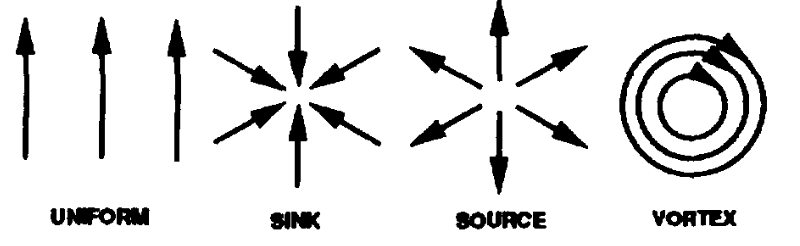
\includegraphics[width = .8\linewidth]{aerodynamics-primitives-Wejchert1991.png}
%     % 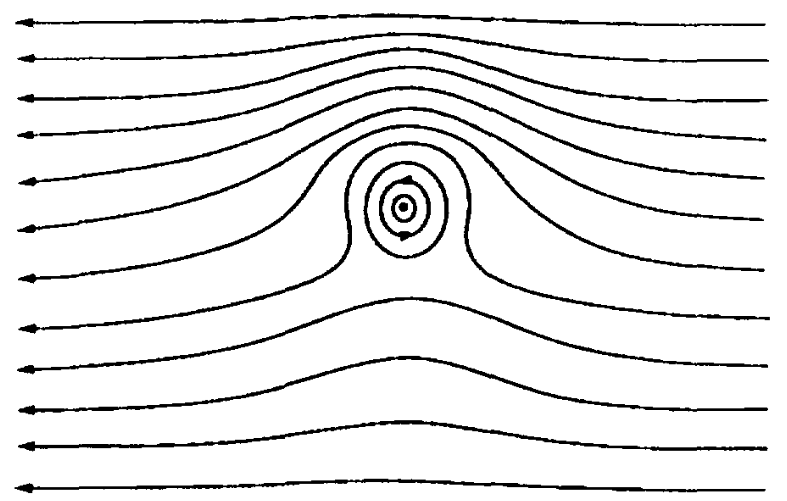
\includegraphics[width = .15\linewidth]{aerodynamics-addition-Wejchert1991.png}
%     \caption{\cite{Wejchert1991} propose to describe the flowfield of the environment by a combination of primitives, resulting in a simulation of wind field controllable by the user at very small memory cost. }
%     \label{fig:env-obj-wejchert-flow}
% \end{figure}

% \begin{figure}
%     \autofitgraphics[]{riverscape-primitives-Peytavie2019.png, riverscape-result-Peytavie2019.png}
%     \caption{\cite{Peytavie2019} uses a sparse representation of a river surface to include details at the water surface.}
%     \label{fig:env-obj-peytavie-river-primitives}
% \end{figure}

\AltTextImage{
    $\Wobj$ is a deformation field defined as the accumulation of flow primitives. The use of analytical primitives to represent localised variations within large-scale scenes has been explored in various contexts through the edition of wind fields (\cite{Wejchert1991}, \cref{fig:env-obj-wejchert-flow}) and authoring of rivers' water surface geometry (\cite{Peytavie2019}, \cref{fig:env-obj-peytavie-river-primitives}). In the latter, flow primitives are primarily used to generate the geometry of the water surface, but the same primitives can also be reused to produce a flow field, enabling effects such as floating debris or leaves drifting along the surface. Because geometry is sensitive to overlapping influences, the authors organise primitives into a blending tree, where merge and replace operations control how individual contributions interact.
}{riverscape-primitives-Peytavie2019.png, riverscape-result-Peytavie2019.png}{\cite{Peytavie2019} uses a sparse representation of a river surface to include details at the water surface that can be aggregated in a construction tree.}{fig:env-obj-peytavie-river-primitives}

\AltTextImage{
    On the other hand, \cite{Wejchert1991} showed that simply summing flow primitives generates velocity fields that approximate Navier-Stokes dynamics (\cref{fig:env-obj-wejchert-flow}, bottom). Because their method affects motion rather than visible geometry, this additive approach offers a good trade-off between plausibility, user control, and computation time.
    In our method, we adopt a similar additive approach to combine Kelvinlet-based primitives. Our goal is to define a deformation field, and as such, summation offers an effective and intuitive way to accumulate the influence of multiple localised deformations at various scales, without requiring additional structure to resolve overlaps.  
}{aerodynamics-primitives-Wejchert1991.png, aerodynamics-addition-Wejchert1991.png}{\cite{Wejchert1991} propose to describe the flow field of the environment by a sum of primitives, resulting in a simulation of wind field controllable by the user at very small memory cost.}{fig:env-obj-wejchert-flow}
% To model the localized influence of environment objects on water currents, we adopt Kelvinlets, a family of closed-form, continuous deformation functions derived from the fundamental solutions to the equations of linear elasticity in an infinite medium.


% \begin{figure}
%     \autofitgraphics[]{kelvinlets-grab-demo-DeGoes2017.png, kelvinlets-demo-DeGoes2017.png}
%     \caption{\cite{DeGoes2017} presents four types of deformations using Kelvinets, resulting in organic pinch-like interaction with the original field. From left to right: a grab on a \textcopyright Disney/Pixar character, a twist, a scale and a pinch operation. }
%     \label{fig:env-obj-kelvinlets-demo}
% \end{figure}

Kelvinlets were introduced to computer graphics as an efficient means of producing physically plausible and interactive deformations \cite{DeGoes2017}. In our context, they provide a smooth and compact representation of flow alterations, ideal for integrating environmental features into vector field modelling.

Kelvinlets are based on the Kelvin solution, which is the Green's function of the Navier-Cauchy equations of linear elasticity. It describes the displacement $\tensor{u}(\p)$ at a point $\p \in \R^3$ caused by a force applied at $\q$, in an isotropic, homogeneous elastic material:
\begin{align}
    \mu \nabla^2 \tensor{u} + (\lambda + \mu) \nabla(\nabla \cdot \tensor{u}) + \delta(\p - \q) \force = 0
\end{align}
where $\lambda$ and $\mu$ are the Lamé parameters, with $\mu$ also known as the shear modulus, and $\force$ is the force vector applied at a single point $\q$ via the Dirac delta function $\delta(\p - \q)$.

\AltTextImage{
    To regularise the singularity at $\p = \q$, \cite{DeGoes2017} introduced a smoothed form known as the regularised Kelvinlets, which allow deformation effects to fall off smoothly with distance, and prevent numerical instabilities.
    Given a centre $\q$, an evaluation point $\p$, and a regularisation $\eps$, we define $\tensor{r} = \p - \q$ and the regularised distance $r_{\eps} = \sqrt{\|\tensor{r}\|^2 + \eps^2}$.

    We use the scale and grab formulations of the regularised Kelvinlets brushes (\cref{fig:env-obj-kelvinlets-demo}), denoted as $s_\eps(\tensor{r})$ and $g_\eps(\tensor{r})$ respectively, to simulate obstruction and diversion, and define them as
    \begin{align*}
        s_\eps(\tensor{r}) &= (2b - a) \left( \frac{1}{r_\eps^3} + \frac{1}{2r_\eps^5} \right)(s \tensor{r}) \\
        g_\eps(\tensor{r}) &= \left[ \frac{a - b}{r_\eps} \identity + \frac{b}{r_\eps^3} \tensor{r} \tensor{r}^t + 
    \frac{a \eps^2}{2 r_\eps^3} \identity \right] \force
    \end{align*}
    with $a = \frac{1}{4 \pi \mu}$ and $b = \frac{a}{4 (1 - \upsilon)}$, provided $\mu$ is a shear modulus and $\upsilon$ a Poisson ratio specified for each Kelvinlet, $s$ a scaling factor, and $\force$ the force vector of the grab operation. These values are tunable per object to simulate different material or flow resistance behaviours.
}{kelvinlets-grab-demo-DeGoes2017.png, kelvinlets-demo-DeGoes2017.png}{\cite{DeGoes2017} presents four types of deformations using Kelvinlets, resulting in organic pinch-like interaction with the original field. Top: a grab on a \textcopyright Disney/Pixar character. Bottom, from left to right: a twist, a scale, and a pinch operation.}{fig:env-obj-kelvinlets-demo}

Deformations defined on curves use $\q = \closestCp$ with $\closestCp$ the closest point on the curve from the point $\p$ and $\force = \curve'(\p)$. We can then define $\tensor{u}o(\p) = s\eps(\q - \p) + g_\eps(\p - \q)$.

Finally, we retrieve the velocity field from the objects, with a per-object coefficient $\lambda_o$ for the strength of its flow effects (due to its size, porosity, surface roughness, etc.):
\begin{align}
    \Wobj(\p) = \sum_{o \in \objects}^{}{\lambda_o \tensor{u}_o(\p)}
\end{align}

The use of regularised Kelvinlets is well-suited to our model. They offer a compact representation thanks to their closed-form definition, which allows each deformation to be described analytically without the need for precomputed data or large simulation grids. They maintain continuity, ensuring that the resulting vector field is smooth and free of visual or numerical artefacts, which is crucial when blending influences from multiple environment objects. Their behaviour is physically plausible, as they are derived from fundamental solutions to elasticity equations, and can convincingly simulate natural flow behaviours such as deflection around obstacles or local flow obstruction. They are also computationally efficient, since their evaluation is lightweight and independent of the size or complexity of the terrain, making them particularly suitable for integration into large-scale procedural generation pipelines and real-time interactive applications.

\cref{fig:env-obj-rock-with-kelvinlets} presents a rock acting as an obstacle to the incoming water flow, which guides the flow, and more importantly the \glosses{EnvMat}, in a plausible direction on the side of the obstacle, with the introduction of artificial vortices at its back. A curve-based water influence is presented in \cref{fig:env-obj-canyon-flow}, which is a unique "grab Kelvinlet" in the direction of the curve skeleton of the canyon.

Unfortunately, the Kelvinlet paradigm is not applicable to region-based \glosses{EnvObj}. In this case, the water influence is given using the vector towards the closest point on the outline, scaled by the distance between the evaluation point and the curve, as presented in \cref{fig:env-obj-island-flowfield}. Note that the vector field produced by the islands is directly computed by the distance field of its region's boundaries and is independent of the generated geometry, explaining the discrepancy between the emerged surface and the resulting flow field in \cref{fig:env-obj-island-flowfield}.

\begin{figure}
\autofitgraphics[]{2025-06-21__12-53-48_render_top_view-with-sand.png, 2025-06-21__12-53-48_render_top_view-with-flow-with-sand.png, 2025-06-21__12-53-48_render_top_view-with-flow-with-sand-with-annotations.png}
\caption{A strong current is affected by a rock, visible by the deviation of sand (green) produced by smaller rocks. The flow is directly computed by the composition of three Kelvinlet objects assigned to the rock: a "scale Kelvinlet" (yellow) deflects the materials as an obstacle would; and two "twist Kelvinlets" (cyan) approximate the vortices of the flow, pushing the sand back behind the rock.}
\label{fig:env-obj-rock-with-kelvinlets}
\end{figure}

\begin{figure}
    \autofitgraphics[]{2025-06-20__08-57-28_render_top_view-no-flow.png, 2025-06-20__08-57-45_render_top_view-no-flow.png, 2025-06-20__08-58-02_render_top_view-no-flow.png}
    \autofitgraphics[]{2025-06-20__08-57-28_render_top_view-with-flow.png, 2025-06-20__08-57-45_render_top_view-with-flow.png, 2025-06-20__08-58-02_render_top_view-with-flow.png}
    \caption{Each \gloss{EnvObj} has an influence on the water currents. Islands, defined with an area, add a force towards themselves (waves crashing on coasts) and simultaneously a force towards the ocean that acts as an obstacle flow. The resulting vector field of the scene is the sum of each \gloss{EnvObj}'s influence.}
    \label{fig:env-obj-island-flowfield}
\end{figure}

% \subsection{Environment stability}
% \begin{figure}[H]
%     \centering
%     \autofitgraphics[]{diffusion_no_decay_no_wind.pdf, diffusion_decay_0-05_no_wind.pdf}
%     % \autofitgraphics[]{diffusion_no_decay_linear_wind.pdf, diffusion_decay_0-05_linear_wind.pdf}
%     \autofitgraphics[]{diffusion_no_decay_circular_wind.pdf, diffusion_decay_0-05_circular_wind.pdf}
%     \caption{The addition of a decay term in the advection-diffusion-reaction equation, the spread of the \glosses{EnvMat} tends to a stability after few iterations (right) while the total mass would constantly increase without decay (left) (concentration value is clamped to 1 for visual purposes). This is also true when a flow field is present (bottom). Moreover, thanks to the decay, we see less instabilities regarding the boundary conditions (bottom left uses a zero-gradient boundary condition, resulting in a simulation explosion from the borders). }
%     \label{fig:env-obj-stability-examples}
% \end{figure}

% \Glosses{EnvObj} and \glosses{EnvMat} are inspired by the ecological concept of biogeocoenosis, which describes the relationship between living organisms (biotic) and their non-living environment (abiotic). These interactions closely mirror the processes observed in natural ecosystems, where biotic and abiotic components continuously influence each other, leading to a balanced and stable environment. Gubanov and Degermendzhy [CITATION] describe biogeocoenosis as almost-closed systems, with many parallels possible with thermodynamics such as the concept of dynamic equilibrium. In a biogeocoenosis, the various processes, such as the spread of nutrients, the growth of vegetation, or the erosion of soil, tend toward a state of balance. 

% Similarly, in our method, the interaction between \glosses{EnvObj} and \glosses{EnvMat} is modeled using a reaction-diffusion-advection framework. This model captures how \glosses{EnvMat} are spread and absorbed within the terrain. Thanks to the decay rate of the \glosses{EnvMat}, the system progresses toward a dynamic equilibrium, where the distribution of \glosses{EnvMat} stabilizes. This stabilization reflects a state of balance where the rates of spreading and absorption and decay are equal, and the \glosses{EnvVal} become coherent across the landscape. For example, a river might spread sediments downstream, which are gradually absorbed by the surrounding terrain, leading to a stable sediment distribution over time. Similarly, moisture emitted by a forest will eventually reach a balance with the surrounding soil and atmosphere, creating a stable, humid environment.

% The only factor that can disrupt this equilibrium is a change in the \glosses{EnvVal}. Changes such as an increase in temperature, a shift in wind patterns, or the introduction of a new \gloss{EnvObj} can alter the balance, leading to a new phase of interaction and stabilization.


\section{User interactions}
\label{sec:env-obj-interaction}
The user can guide the generation process. The use of simple shapes as \glosses{EnvObj} facilitates the edition of the simulation, as we can interactively add, remove or modify \glosses{EnvObj}, or focus the generation process in a restricted area. Interaction with the \glosses{EnvVal} is also provided as \glosses{GeoEvent}, that the user can invoke during the simulation. While the direct interactions on the \glosses{EnvObj} are instantaneous, the \glosses{GeoEvent} are active over a given duration.

\subsection{Direct interactions with the \glosses{EnvObj}}
\label{sec:env-obj-manual-interaction}
The interactive nature of our simulation enables the user to modify the state of the terrain by manipulating directly the \glosses{EnvObj} of the scene. We assume the modifications are applied between two iterations of the simulation.

Translating an \gloss{EnvObj} is trivial, we simply require evaluating the \gloss{FitnessFunc} of the \glosses{EnvObj} at a translated position to verify that the environment is still suitable for its survival.

The deformation \glosses{EnvObj} can be applied on curve and region \glosses{EnvObj} by displacing directly the control points of the skeleton (\cref{fig:env-obj-user-interaction} deforming a canyon, and \cref{fig:env-obj-island-deformation} editing an island). Many methods may be used for displacing a polygon, such as the use of Kelvinlets, cage deformation, displacement maps, or Gaussian influence. In the scope of this chapter, we will not cover the multiple aspects of curve and polygon deformation. However, as the closed or open geometry shape of the \gloss{Skeleton} changes, it needs to run again the \gloss{FittingFunc} optimisation through our Snake algorithm (\cref{sec:env-obj-generation-rules}).

Locking the vertices from the deformed \gloss{Skeleton} edited manually by the user can be achieved by cancelling the energy $\energy(\curve)_v$ from the Snake algorithm for this specific vertex $v$, disabling it from any displacement during the optimisation process. Finer control can be given by applying a coefficient on the energy gradient, such that the vertices are not locked but hindered.

By modifying an \gloss{EnvObj}, the \glosses{EnvVal} may change, which can result in the destruction of the now incompatible \glosses{EnvObj} in the scene (\cref{fig:env-obj-user-interaction}, middle). The removal of \gloss{EnvObj} is subject to chain reactions, often visible in nature. Reducing the reaction is achievable by alternating, until a steady state is reached again, a step in the environment update (\cref{sec:env-obj-materials}) and a step of \gloss{Skeleton} refinement for each \gloss{EnvObj}. As a counterbalance to the removal, each deleted \gloss{EnvObj} is reinserted in the scene (\cref{fig:env-obj-user-interaction}, right) following the process described in \cref{sec:env-obj-generation-rules}.

\begin{figure}
    \autofitgraphics[]{InteractionEdition1.png, InteractionEdition2.png, InteractionEdition3.png}
    \caption{Starting from a coral colony developed around a canyon (left), the user edits the shape of the canyon, resulting in a different configuration of the scene, killing the corals that end up too deep in the water (centre) and the development and growth of new corals at the previous location of the canyon (right).}
    \label{fig:env-obj-user-interaction}
\end{figure}

As long as a non-zero \gloss{FitnessFunc} is defined in the terrain, new \glosses{EnvObj} can be forced by the user at any point of the simulation.

Control over the region of the terrain that should be updated can be given by adjusting all \glosses{FitnessFunc} through a scalar field $\influence: \R^2 \to \R $ such that the \gloss{FitnessFunc} $\fitnessFunc(\p)$ of any new \gloss{EnvObj} is evaluated as $\fitnessFunc^*(\p) = \influence{\p} \fitnessFunc(\p)$. This is especially useful in the planning of robotic simulations, as we can first generate the overall shape of our terrain and secondly focus the generation process around the areas that may be visited by the robot, avoiding useless simulations and computational power.
\cref{fig:env-obj-coral-colonization-scene} shows an example of colonisation of the coral polyps that we limited manually into an annulus.

Our water current simulation is modelled as a simple vector field. As such, the user is able to interact with it at any moment of the simulation, allowing for the death of sensitive \glosses{EnvObj} while guiding the simulation into a new landscape. By modifying the water currents, the user also modifies the transport rate of \glosses{EnvMat} at this position. The modification of currents is given as a stroke, a parametric curve $\curve$ for which we evaluate $\Delta \Wuser(\p)$ just as described in \cref{chap:coral-island}'s user-driven wind velocity field construction. A simple user stroke shows the impact of a strong underwater current on coral colonies in \cref{fig:env-obj-user-flow-effects}.

\begin{figure}
    \autofitgraphics[]{2025-06-20__00-37-15_render_top_view.png, 2025-06-20__00-37-47_render_top_view.png}
    \caption{Deformation of an \gloss{EnvObj} is applied by displacing the control points of its outlines. All \glosses{EnvObj} in the scene evaluate their new fitness in the environment.}
    \label{fig:env-obj-island-deformation}
\end{figure}

\begin{figure}
    \autofitgraphics[]{2025-06-20__02-00-57_render_top_view.png, 2025-06-20__02-01-59_render_top_view.png}
    \caption{A strong water current created by the user has a direct influence on the corals that are sensitive. \Glosses{EnvObj} that are far enough from the user stroke are unaffected.}
    \label{fig:env-obj-user-flow-effects}
\end{figure}

\subsection{Indirect interaction with \glosses{EnvObj}}
\label{sec:env-obj-events}
A configuration file can define in advance the different \glosses{GeoEvent} that should be triggered during the simulation. This can be useful to generate landscapes that are close to some existing locations.
Multiple \glosses{GeoEvent} can be triggered either as sudden or continuous environmental changes. These changes play a huge role in the morphology of landscapes.
We define \glosses{GeoEvent} with a starting point and an ending point, such that at any time of the simulation we can compute the progress of the \gloss{GeoEvent} as $\tEvent \in [0, 1]$ and linearly interpolate the effects on \glosses{EnvVal}.

\subsubsection{Water level events}
Water level changes are important \glosses{GeoEvent} that shape underwater landscapes. As previously submerged \glosses{EnvObj} become elevated above the water level, flora and fauna terrain features dry and die. Deprived of the living part of the features, everything is more affected by terrestrial erosion. By updating the value of the depth $\depth$ evaluated in the \glosses{FitnessFunc}, any \gloss{EnvObj} that is sensitive to depth and altitude will be impacted automatically, which may cause death (\cref{fig:env-obj-water-event}). The modification of the water level is defined as
\begin{align}
    \depth(\p) = \depth_0(\p) + \sum_{e \in \events} \Delta \depth_e \tEvent
\end{align}
with $\Delta \depth_e$ the amount of water rising or lowering during a \gloss{GeoEvent}. We assume a linear evolution of the water level during a \gloss{GeoEvent}. This allows the evaluation of depth at any point in space and time.

\begin{figure}
    \autofitgraphics[]{InteractionWater1.png, InteractionWater3.png}
    \caption{Lowering the water level by a few metres caused most of the coral objects to satisfy $\fitnessFunc \leq 0$, causing their death. Since the water level (blue) decreases slowly, new coral objects spawn progressively at a lower altitude.}
    \label{fig:env-obj-water-event}
\end{figure}

\subsubsection{Subsidence and uplift events}
Subsidence and uplift are the main \glosses{GeoEvent} that create or destroy islands in the long term, as presented in \cref{chap:coral-island}. These \glosses{GeoEvent} are simulated as a simple factor on the height field of the generated terrain (\cref{fig:env-obj-subsidence-event}). Subsidence is not always uniform across the terrain. As such, the user can provide a position $\q$ at which the subsidence is strongest, the amount of subsidence applied $\Delta \height_e$ and a standard deviation $\std$, from which we can then compute, at any point in space and time of the simulation, the height of the terrain:
\begin{align*}
    \height(\p) = \height_0(\p) \cdot \sum_{e \in \events}{G(\norm{\p - \q})} \Delta \height_e \tEvent
\end{align*}
with $G_{\std}(x)$ the Gaussian function
\begin{align}
    G_{\std}(x) = \frac{1}{\std \sqrt{2\pi}} \exp \left(-\frac {x^{2}}{2 \std ^{2}}\right)
\end{align}
The Gaussian formulation guarantees continuity and an analytic formulation of the changes on the \glosses{EnvVal}, with smooth transitions from the epicentre of the \glosses{GeoEvent} as the distance increases. Any other analytical formulation could be used, but the Gaussian formulation has been chosen as the only parameter needing tuning by the user is the standard deviation $\std$.

\begin{figure}
    \autofitgraphics[]{InteractionSubsidence1.png, InteractionSubsidence2.png}
    \caption{Simulating subsidence on a part of the terrain (brown area) causes the depth value to change locally, resulting in the death of coral objects that find themselves too deep to survive. Here two subsidence \glosses{GeoEvent} are triggered in parallel.}
    \label{fig:env-obj-subsidence-event}
\end{figure}

\subsubsection{Storm events}
Storms are factors in the geomorphology of coral reefs \cite{VilaConcejo2016, Oron2023} and coasts \cite{Dominguez2005, Cowart2010}. Due to the extreme wind and wave velocities, coasts are highly eroded in a short time period and the more fragile corals near the water surface are broken, possibly causing breaches in the reefs and spreading polyps in the current's direction. While there are many factors at play to understand the appearance of storms and the hydrodynamics affecting them, we simplified the model of storms for the user to a single epicentre $\q$ with a wind velocity $\windVelocity$ and a standard deviation $\std$ representing the spread around the epicentre (\cref{fig:env-obj-storm-event}). The computation of water currents is then given as
\begin{align*}
    \Wuser(\p) = \Wuser^*(\p) + \sum_{e \in \events} {\windVelocity G(\norm{\p - \q})}
\end{align*}
In this case, we did not include the linear factor $\tEvent$ as storms are usually conserving a constant force for the time of the few weeks or months of their occurrence. 

\begin{figure}
    \autofitgraphics[]{interactionStorm1.png, interactionStorm2.png}
    \caption{The result of a storm localised on one side of the island (red area) modifies the result of the evaluation of \glosses{EnvObj} around its epicentre for a short period of time. Most of the coral objects died from the \gloss{GeoEvent}, except for a few \glosses{EnvObj} less sensitive to the strength of the water currents.}
    \label{fig:env-obj-storm-event}
\end{figure}

% Just as for the rise and lowering of water level, the heat is modeled as a simple value of the environment. For shallow areas (<100m) we assume a linear relation between depth and temperature, and a constant value for the terrestrial environment. As such, we can model a heat wave by a change of the \glosses{EnvVal}. \Glosses{EnvObj} who are sensible to temperature may die instantly. The modification of the temperature is defined as 
% \begin{align*}
%     \temperature(\p) = T_0(\p) + \sum_{e \in \events} \Delta \temperature_e \tEvent + c \depth(\p)
% \end{align*}
with $\Delta \temperature_e$ the change of heat during an \gloss{GeoEvent}, $\temperature_0$ the temperature at the water surface, and $c$ a very small factor.

\midConclusion

The framework can easily be extended as the \gloss{GeoEvent} system remains similar for all \glosses{GeoEvent}. Including higher-level simulations in the \gloss{GeoEvent} system can be added, such as the simulation of tectonic activity, the use of fluid dynamics for tsunami \glosses{GeoEvent}, the integration of human activity, etc...

\section{Results and discussion}
\label{sec:env-obj-results}
Our method provides a way to generate scenes at different scales. We demonstrate this capacity with the generation of a large scene of an island (\cref{fig:env-obj-teaser}), after which we focused the generation process in a canyon (\cref{fig:env-obj-canyon-scene}), then a small-scale visualisation of coral colonies (\cref{fig:env-obj-coral-colonization-scene}).
In the examples, we rendered the \glosses{EnvObj} as an implicit tree or as individual meshes. The island, lagoons, reefs, canyons and sand ripples as implicit surfaces.

\begin{figure}
    \autofitgraphics[]{2025-06-20__10-32-20_render_top_view.png , 2025-06-20__10-32-20_render_top_view-with-flow.png }
    \caption{A canyon creates a water current in its direction.}
    \label{fig:env-obj-canyon-flow}
\end{figure}

\begin{figure}
    \autofitgraphics[]{2025-06-20__10-32-42_render_inside_view.png, 2025-06-20__10-33-11_render_inside_view-with-boulders.png, 2025-06-20__10-33-11_render_inside_view-with-shade.png, 2025-06-20__10-36-21_render_inside_view-with-sand.png}
    \caption{Inside view of a canyon with an arch. The arch generates shade (red) and pebbles (green), which is a beneficial environment for the appearance of rocks, which will in turn spread sand.}
    \label{fig:env-obj-canyon-inside-with-arch}
\end{figure}

\begin{figure}
    \autofitgraphics[]{2025-06-20__10-36-21_render_top_view-with-sand.png, 2025-06-20__10-38-05_render_top_view-with-sand-small-decay.png, 2025-06-20__10-39-13_render_top_view-with-sand-no-water-transport.png}
    \autofitgraphics[]{2025-06-20__10-40-44_render_top_view-with-sand-high-diffusion.png, 2025-06-20__10-42-22_render_top_view-with-sand-reverse-water-transport.png }
    \caption{Influence of material parameters on their spread (sand generated by the rocks). From left to right, and top to bottom: normal sand parameters, low decay, no influence of water flow, large diffusivity, inverse water influence (spread upwind in the canyon).}
    \label{fig:env-obj-material-diffusion-parameters}
\end{figure}

\begin{figure}
    \autofitgraphics[]{2025-06-20__15-54-59_render_top_view-with-flow-with-sand.png, 2025-06-20__15-57-26_render_top_view-with-sand.png, 2025-06-20__15-58-34_render_top_view-with-sand.png, 2025-06-20__16-01-26_render_top_view-with-deadcoral.png,
    2025-06-20__16-04-20_render_top_view-with-deadcoral.png}
    \autofitgraphics[]{2025-06-20__15-54-59_input_label.png, 2025-06-20__15-54-59_input_label.png, 2025-06-20__15-57-26_input_label.png, 2025-06-20__15-58-34_input_label.png,
    2025-06-20__16-04-20_input_label.png}
    \caption{Iterative construction of an island under high wind force, the deposition of sand is affected by the wind, giving an elongated shape to the beach. The large presence of sand due to the beach creates a lagoon, and quickly coral colonies spread on the borders of the lagoon to avoid the sand. Coral reefs appear from the deposition of calcareous material from coral. Bottom: The label map used in \cref{chap:coral-island} can be extracted from the \glosses{EnvObj} of the scene.}
    \label{fig:env-obj-iterative-island}
\end{figure}

A canyon scene can be generated using our method. The water flow is affected by the curve of the canyon such that the currents are oriented in the direction of the curve's tangent. In this example, we force the position of arches to be inside the canyon. The arches deposit a material "rock deposit", which is the main element of the \gloss{FitnessFunc} of the Rock object. The "rock deposit" is slightly affected by water currents, but its mass makes it highly affected by gravity. As such, rocks will spawn underneath arches. In reality, an arch is often created as part of a large coral boulder that sees the calcareous bottom part detached by the water currents, often resulting in an arch surrounded by big rocks and smaller rocks from the erosion of the first rocks.

As such, we define an \gloss{EnvObj} "Arch" with a \gloss{FitnessFunc} $\fitnessFunc_{arch}(\p) = 5 - d(canyon - \p) * \norm{\Water(\p)}$, an \gloss{EnvObj} "Rock" using $\fitnessFunc_{rock}(\p) = \material_{rock\_deposit}(\p)$ and Pebble using $\fitnessFunc_{pebble}(\p) = \material_{smaller\_rock\_deposit}(\p)$. Finally, sand ripples are simply described as curves appearing where there is a lot of sand available: $\fitnessFunc_{ripple}(\p) = \material_{sand}(\p)$.

Following these simple rules, \cref{fig:env-obj-canyon-scene} shows the emergence of details in the scene.

\begin{figure}
    \autofitgraphics[]{Canyon2.png, Canyon3.png, Canyon4.png, Canyon5.png}
    \caption{Evolution of a canyon scene at different iterations of the simulation. The appearance of an arch causes the spawning of rocks, pebbles, and finally some deposition of sand at the bottom of the canyon, spawning ripples.}
    \label{fig:env-obj-canyon-scene}
\end{figure}

% \subsection{Small-scale}
% \label{sec:env-obj-small-scale}
In this example we defined three different types of corals, coralA, coralB and coralC, to illustrate the possibility to model behaviours from the choice of \glosses{FitnessFunc}. Each of the coral types deposits a material "coral polyp" and "coral polyp A" ("coral polyp B" and "coral polyp \curve" respectively). By considering a \gloss{FitnessFunc} that minimises the ratio $\frac{\text{coral polyp}}{\text{coral polyp A}}$, we can see an emergent behaviour of the three types of coral fighting for the space colonisation.
\cref{fig:env-obj-coral-colonization-scene} shows the result of this simulation at three different iterations. At the border between two colonies, none of the colonies make progression due to the amount of coral polyp specific from the other colony.

\begin{figure}
    \autofitgraphics[]{focusArea.png, col0.png, col1.png, col2.png, col3.png}
    \caption{Three colonies of coral (red, blue, green) restricted to an annulus (leftmost, red has negative impact on the fitness function while green has positive impact) in the middle section of the terrain fighting for the space.}
    \label{fig:env-obj-coral-colonization-scene}
\end{figure}

\begin{figure}
    \autofitgraphics{islands_with_different_coral_types.png}
    \caption{Introducing penalities on water currents and terrain slope for different types of corals, we see naturally a layout emerging with branching corals (purple) in the back reef, foliose corals (cyan) mainly around the reef crest, and massive corals (brown) spreading from the back reef to the fore reef. }
    \label{fig:env-obj-coral-layout}
\end{figure}

The proposed method aims to generate plausible landscapes using simplified versions of the evolution of an ecosystem and of the 3D representation. The biological realism of the result is highly correlated to the amount of simplification and assumptions, while the visual realism is completely dependent on the geometric functions used for the 3D modelling of the \glosses{EnvObj}. While proposing a flexible method that proposes a generic approach for terrain generation, a close collaboration with field experts and with graphists is needed to achieve optimal results. Adding notions of slope and sensibility to water currents in \cref{fig:env-obj-coral-layout} for different coral morphologies (massive, branching, foliose and table corals), each coral entity finds a place that fits the distribution of species presented in \cref{sec:state-of-the-art_biology}. 

Most simulation algorithm's quality depends on the size of the time step used, but with the introduction of a decay rate in the \glosses{EnvMat} properties, we limit the influence of time steps by considering that steady states are reachable. The material deposition and absorption on punctual \glosses{EnvObj} can be seen as a Dirac function $\dirac$ centred at their position, resulting in the advantage that material displacement function can use the definition of the diffusion equation instead of the advection-diffusion-reaction equation. This equation allows us to evaluate the state of the material $\material$ without intermediate steps, but this is not applicable with curve- and region-based \glosses{EnvObj}.


\section{Conclusion}
\label{sec:env-obj-conclusion}
We have proposed a method to generate terrains procedurally using sparse representations. This representation, the \glosses{EnvObj}, enables the introduction of expert knowledge by the means of the \glosses{FitnessFunc} that rule the \glosses{EnvObj} life cycle, but also to integrate the user in the loop during the generation process. We reduced the terrain resolution limitations by defining the environment objects as parametric features. Thanks to the sparse representation based on single points, curves and regions, we allow for direct manipulation of the \glosses{EnvObj} of the scene by the user which, thanks to the environment steady state consideration, also enables these interactions to be included in the automatic simulation process.

Integrating environmental properties in the \gloss{FitnessFunc} of \glosses{EnvObj} allows the user to guide the generation through \glosses{GeoEvent}. Our method enables each \gloss{EnvObj} of the scene to influence the environment locally, reducing the need for computations while also retrieving \glosses{EnvVal} locally, which results in a parallelisable life-like simulation process. The genericity of the environment properties definitions should be sufficient for plausible generation of other landscape types as long as expert knowledge can be translated to \gloss{EnvObj}'s formalism.

We limited our work to the use of 2D scalar fields as they are more easily differentiable, interpretable and lighter than volumetric representations. However, future works include using 3D representations of the terrain and the environment to generate 3D terrains, including cavities, sub-terrestrial areas and the interior of coral structures.

\begin{figure}[H]
    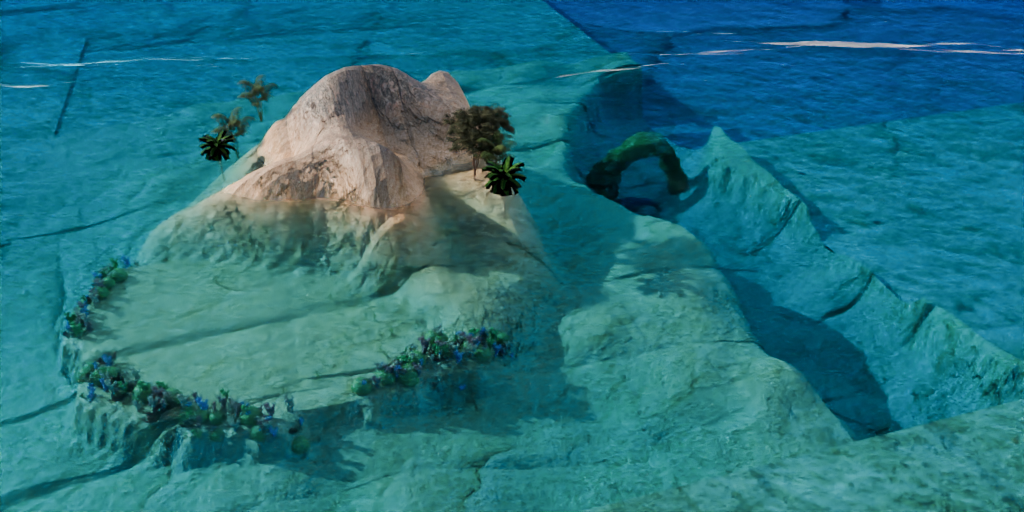
\includegraphics{multiScene1 v2 final 1.png}
    \caption{A simple coral reef island is generated using an island, a lagoon, reefs, coral polyps, beaches, trees and algae \glosses{EnvObj}. Trees appear on beaches and algae grow in the lagoon's sand.}
    \label{fig:env-obj-coral-island-scene}
\end{figure}



















% \section{Method}
% \label{sec:env-obj-method}
% The overall pipeline of the method is based on simple incremental generation such as most rule-based systems. In this type of system, the final state is defined either by reaching equilibrium, or by verifying specific conditions, such as a maximum number of iterations. 
% We define our pipeline in three phases (\cref{fig:env-obj-pipeline}): the initialization phase that describe the generation and simulation rules, the iterative phase generating populating the terrain with our \glosses{EnvObj} and finally the output.


% \subsection{Pipeline overview}





















% \section{Expert knowledge integration}
% \label{sec:env-obj-biology}
%   The definition of the \glosses{FitnessFunc} of the \glosses{EnvObj} are inspired by the biological and geological factors that rule the evolution of underwater landscapes. The main factors are depth, light, water currents and biodiversity. External \glosses{GeoEvent} have direct and indirect repercussions on the biodiversity of underwater environments. Coral reef islands are complex bio systems in which fauna, flora and geology are mixed together. 

% \subsection{\Glosses{EnvObj} description}
% \label{sec:env-obj-represented-objects}
% We have represented with \glosses{EnvObj} some geologic features, animal features and flora features. The low island is most often raised in a circular shape as the process mainly appear around a hot spot under the ground. The evolution of an island into a coral reef island requires that the environmental conditions are sufficient for coral development: corals will grow slightly below the water surface as waves will break its growth and at a shallow depth (around 3m to 30m deep) in order for light to reach it. As coral grow and die, the skeleton is transformed into porous limestone, providing shelter to surrounding animals and reducing the impact of water erosion on the island. Corals drop polyps that are transported by the water flow and when they stick to a hard surface, as a rock or the reef itself, the coral may grow and colonize the area. As subsidence cause the island to lower, the living part of the coral reef keep growing toward light, which lead to a reef that is constantly close to the water level without reaching it due to wave erosion. The survival of reefs depends on the equilibrium between coral growth and and erosion. Eroded parts of the reef falling in the sheltered part of the reef accumulates, ending up by forming a lagoon. An island formed by a hot spot will inevitably subside in time, until it is completely flatten. As the coral reefs keep growing, only the lagoon remain, resulting in an atoll. \\
% In this work we we integrate the biological and geological knowledge in the \glosses{FitnessFunc} of the \glosses{EnvObj} we want to generate. We represent the islands as regions that can be appearing with a uniform distribution. From the formulation of the region description \eqref{eq:env-obj-snake-energy-equation}, we mostly create circular islands. The coral features, \glosses{EnvObj} described as a single point, have a \gloss{FitnessFunc} that take into account the depth of the ground, the amount of sand, fresh water and polyps in their environment, as well as the strength of water currents. Each coral species have different living conditions, but we reduced our work to soft coral which are sensible to water strength and stony corals that are more resistant to erosion. Reefs are formed as coral's skeleton are transformed into calcareous stone, describing then as an \gloss{EnvObj} representing multiple others. 

% \subsection{Simplifications}
% \label{sec:env-obj-simplifications}
% The environmental factors simulated are greatly simplified as the real processes are in a very small time scale, that computer simulation are not able to simulate in interactive time. The use of \glosses{EnvObj} aim to represent a plausible results, while avoiding modeling the smaller scale \glosses{GeoEvent}. Examples of simplifications are the geometry and material of each \gloss{EnvObj}, which have an influence on the water currents through friction, the water currents represented as stationary flows, while the water flow dynamics are a complex system that may change completely at two different times of the day, the animal influence on the reefs that they transform by the ingestion and deposition of sediments, ...
